\documentclass{article}
\usepackage{stackengine}
%\usepackage[utf8]{inputenc}
\usepackage[T1]{fontenc}
\usepackage{amsmath}
\usepackage{amsfonts}
\usepackage{graphicx}
\usepackage{pbsi}
\usepackage{lmodern}
%\usepackage{tgbonum}
\usepackage{rotating}
\usepackage{pdflscape}
%\usepackage[a5paper]{geometry}
\usepackage[a5paper, inner=2cm,outer=2.8cm, twoside, bottom=3.2cm]{geometry}
%\usepackage[paperwidth=5.5in, paperheight=8.5in]{geometry}
\usepackage{pdfpages}



%\newwrite\file
%\immediate\openout\file=myfilename.txt
%\immediate\write\file{A line of text to write to the file}
%\immediate\write\file{Another line of text to write to the file}
%\closeout\file

\usepackage{tikz}
\usetikzlibrary{calc}
\newcommand*{\vertchar}[2][0pt]{%
  \tikz[
    inner sep=1pt,
    shorten >=-.15ex,
    shorten <=-.15ex,
    line cap=round,
    baseline=(c.base),
  ]\draw
    (0,0) node (c) {#2}
    ($(c.north)+(#1,0)$) -- ($(c.north)+(#1,0)$);%
}


\makeatletter
\newcommand{\dotr}[1]{%
  \mathpalette\@dotr{#1}%
}

\newcommand*{\@dotr}[2]{%
  % #1: math style (\displaystyle, ..., \scriptscriptstyle)
  % #2: argument of \dotr
  \sbox0{$\m@th#1#2$}%
  \usebox{0}%
  % simulating a superscript
  %\raisebox{\dimexpr\ht0-\height}{$\m@th#1\addvbuffer[-1ex 0.9ex]{.}}%
  \raisebox{3.5pt}{$\m@th#1\@smallbullet#1\bullet$}%
  \kern\scriptspace
}
\newcommand*{\@smallbullet}[2]{%
  \scalebox{.3}{$\m@th#1#2$}%
}
\makeatother
    
\newcommand*{\siin}[1]{\stackinset{c}{}{b}{5.5pt}{\small\ttfamily\char'15}{#1}}
\newcommand*{\nn}{\textsuperscript{n}}
\newcommand*{\pehinbsiit}[1]{\stackinset{c}{}{b}{5.5pt}{\hspace{-2pt}\raisebox{2.5pt}{\begin{rotate}{-35}\small\ttfamily\char'15\end{rotate}}}{#1}}
\newcommand*{\pehinsfit}[1]{\stackinset{c}{}{b}{5.5pt}{\hspace{2pt}\raisebox{2pt}{\small\ttfamily\char'15}}{#1}}
\newcommand*{\pehinrmit}[1]{\stackinset{c}{}{b}{5.5pt}{\hspace{2.5pt}\raisebox{2pt}{\small\ttfamily\char'15}}{#1}}
\newcommand*{\pehin}[1]{\stackinset{c}{}{b}{5.5pt}{\small\ttfamily\char'15}{#1}}
\newcommand*{\pehinbf}[1]{\stackinset{c}{}{b}{5.5pt}{\ttfamily\char'15}{#1}}

\newcommand*{\dtr}{\raisebox{3.5pt}{$\scalebox{.3}{$\bullet$}$}}
\newcommand*{\dtrit}{\hspace{.7pt}\raisebox{3.5pt}{$\scalebox{.3}{$\bullet$}$}}
\newcommand*{\dtrbf}{\raisebox{3.5pt}{$\scalebox{.5}{$\bullet$}$}}



\begin{document}
\pagenumbering{gobble} 
\pagenumbering{arabic}
%\begin{landscape}

\includepdf[pages=-]{untitled-55}
%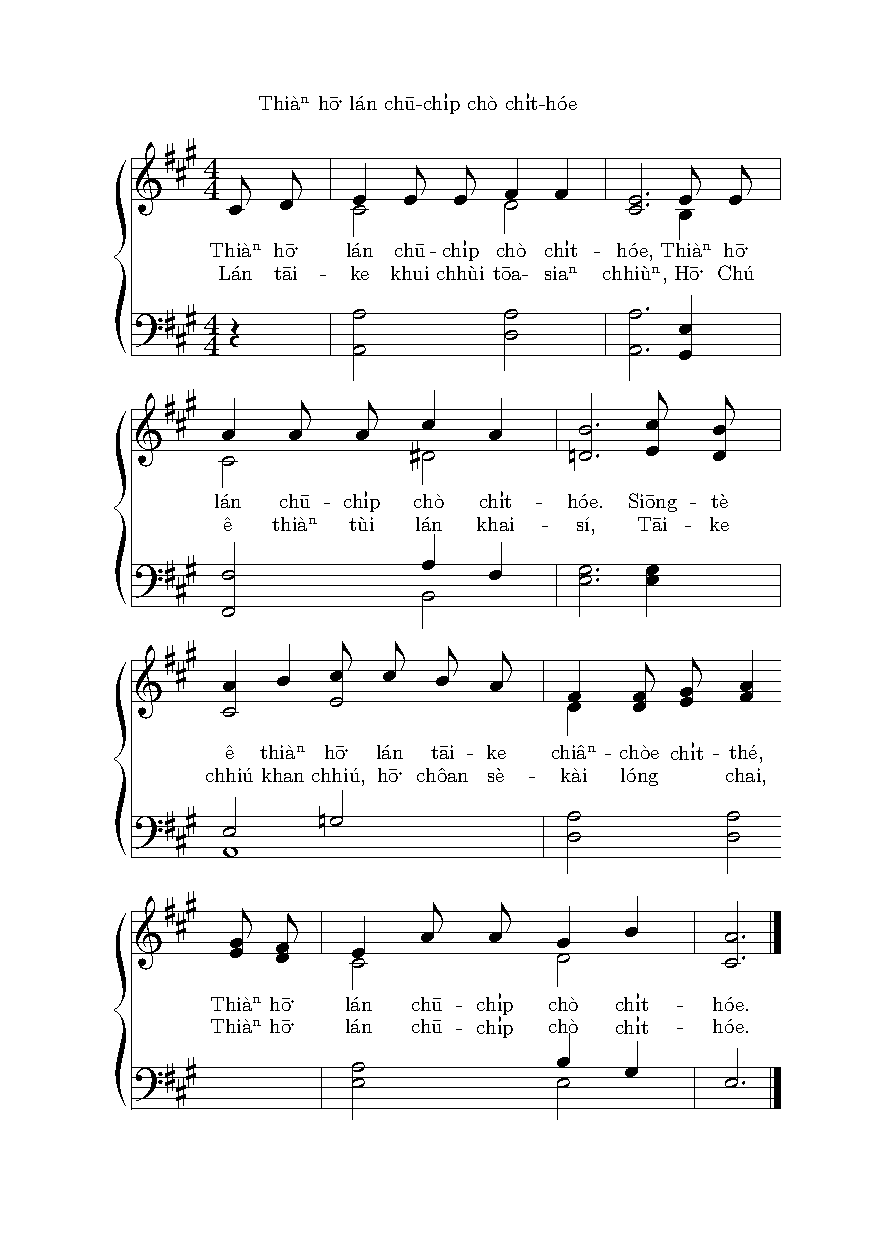
\includepdf[pages=-]{untitled-56}

{\rmfamily
\begin{center}B\pehin{o}k-Li\pehin{o}k\end{center}
\par 
\noindent
\par 6 Ch\'{a}-kh\'{\i} \dotfill 3 \newline
Chheng-ch\'{a} sim-s\^{\i}n kap j\siin{\i}t p\^{\i}{\nn} kh\'{\i} \newline %\dotfill 3 
Go\'{a}n \^{e} Thi{\nn} P\={e} Si\={o}ng-t\`{e} \\%\dotfill\\
Thi{\nn}-kng j\siin{\i}t-chhut \={m}-thang \`{a}i kh\`{u}n \\%\dotfill\\
M\'{u}i ch\'{a}-kh\'{\i} l\'{a}n ti\siin{o}h t\`{\i}-\`{\i} \\ % \dotfill 4\\
I\^{a}-h\^{o}-hoa, ch\'{a}-kh\'{\i}-s\^{\i} \\%\dotfill\\
\noindent
\par 9 Ch\`{o}e-kang \dotfill 5 \newline
Chhut-j\pehin{\i}t l\pehin{o}h-h\={o}{\dtr} s\={\i} Ch\'{u} s\'{o}{\dtr} t\={e}ng \\ %\dotfill 5\\
G\'{o}a \^{e} s\`{\i}n-sim n\={a} b\^{o} ti\={a}{\nn} \\ %\dotfill 4\\
Ch\`{\i} h\'{o} p\^{e}ng-i\'{u} chi\={u}-s\={\i} I\^{a}-s\(\dotr{\text{o}}\) \\%\dotfill\\
G\'{o}a sui \={o}e k\'{o}ng b\={a}n kok im-g\'{u} \\ %\dotfill 6\\ 
B\pehin{o}h-tit tham-ch\^{a}i, kim, g\^{u}n, p\'{o}-kh\`{\i} \\%\dotfill\\
L\'{a}n \^{e} sim-s\^{\i}n ti\pehin{o}h thi\^{a}m-ch\={e}ng \\ %\dotfill 7\\
\noindent
\par 12 J\pehin{\i}t-t\`{a}u \dotfill 7 \\
G\'{o}a him-b\={o}{\dtr} chin-l\'{\i} \^{e} S\^{\i}n \\
Kh\'{u}n-ki\^{u} S\`{e}ng-S\^{\i}n k\'{a}m-t\={o}ng go\'{a}n sim \\%\dotfill\\
Kh\'{u}n-ki\^{u} S\`{e}ng S\^{\i}n k\`{a}ng-l\^{\i}m \\ % \dotfill 8\\
Kh\'{u}n-ki\^{u} S\`{e}ng S\^{\i}n s\`{u} go\'{a}n un-h\={u}i \\%\dotfill\\
\noindent
\par 15 \^{E}-hng \\ \par 18 \`{A}m-m\^{\i} \dotfill 8 \\
Koh k\`{e} ch\pehin{\i}t j\pehin{\i}t s\^{\i}-khek p\^{e}ng-an \\
Ki\^{u} Ch\'{u} kap go\'{a}n t\`{o}a \\ % \dotfill 9\\
Thi{\nn}-p\={e} khi\={a}-kh\'{\i} ch\`{\i}-ko\^{a}n thi{\nn}-t\'{e}ng \\
%Ti\={a}m-ch\={e}ng \`{a}m-m\^{\i} l\={o}{\dtr}-ch\'{u}i teh tih \dotfill 8\\
Sim-l\^{e}ng j\pehin{\i}t-th\^{a}u \\ %\dotfill 10\\
Ch\'{u} s\'{o}{\dtr} h\={o}{\dtr} go\'{a}n ch\pehin{\i}t j\pehin{\i}t ta{\nn} k\`{e}-{-}kh\`{\i} \\ %\dotfill 9\\
\par Ch\'{u}-j\pehin{\i}t \dotfill 12 \\
%Kim-j\pehin{\i}t s\={\i} Ch\'{u} siat-l\pehin{\i}p ch\`{o}e s\`{e}ng \\ %\dotfill 11 \\
%Si\={u} Ch\'{u} si\pehin{o}k-h\^{o}e \\
%T\hspace{.5pt}\={\i} s\pehin{\i}p-j\={\i}-k\`{e} Ki\`{u}-ch\'{u} si\={u} s\'{\i} \\
%Siong-sim si\`{a}u-li\={a}m g\'{o}a Ch\'{u} l\^{a}u-huih \\ %\dotfill 12 \\
%Khek-se-m\'{a}-n\^{\i} hoe-h\^{n}g l\={a}i-b\={\i}n \\
%Ch\'{u} I\^{a}-so{\dtr} p\`{a}ng-sak L\'{\i} p\'{o}-ch\={o} bi\'{a}n-li\^{u} \\
%Ki\`{u}-ch\'{u} thi\`{a}{\nn}-th\`{a}ng \^{e} sia{\nn} \\ %\dotfill 13 \\
%G\={o}a-b\={\i}n phah-m\^{n}g s\={\i} ch\={\i}-ch\={u}i \\ %\dotfill 14 \\
%L\'{\i} ki\'{a}m \={u} chi\={u}-k\={u}n Ch\'{u} h\={o}{\dtr} I s\'{o}e chheng-kh\`{\i} \\ %\dotfill 14 \\
%Si\={o}ng-t\`{e} siat-l\siin{\i}p b\={a}n kok \\ %\dotfill 15 \\
%P\={e}-b\'{u} hia{\nn}-t\={\i} chhin-l\^{a}ng \\ %\dotfill 15 \\
\par K\^{\i}-t\'{o} \dotfill 16 \\
%G\'{o}a bat k\'{o}ng \\%\dotfill 12 \\
%I\^{a}-h\^{o}-hoa s\={\i} g\'{o}a \^{e} kng \\ %\dotfill 16\\
}

\newpage
{\fontfamily{lmr}\selectfont %\rmfamily
%\setlength{\fboxsep}{1cm}
%\fbox{\parbox[t][5cm][t]{\textwidth}{
\par
G\'{o}a \^{e} s\^{\i}n ah, l\'{\i} ti\pehin{o}h cheng-s\^{\i}n kh\'{\i}-l\^{a}i..... Si-phian 57:8 \\
\par
Chheng-ch\'{a} sim-s\^{\i}n kap j\siin{\i}t p\^{\i}{\nn} kh\'{\i}. Che l\^{a}ng h\siin{a}p-s\^{\i} h\'{\i}-l\siin{o}k b\^{o} p\'{\i}. K\`{\i}{\nn}-ti\siin{o}h Si\={o}ng-t\`{e} \^{e}ng-kng \^{e} b\={\i}n. B\={a}n-m\siin{\i}h t\`{u}i I s\^{\i}-si\^{o}ng o\={a}{\nn} sin! 
%\rmfamily
\textsuperscript{2}Si\={o}ng-t\`{e} thi\`{a}{\nn}-th\`{a}ng t\siin{a}k j\siin{\i}t t\^{e}ng-sin. T\`{u}i l\'{a}n kh\`{u}n-chh\'{\i}{\nn} pi\'{a}u-b\^{e}ng s\={\i} chin. Chh\={o}a l\'{a}n p\^{e}ng-an keng-k\`{e} \`{a}m-m\^{\i}. Khoe-h\siin{o}k o\siin{a}h-mi\={a}, kh\`{u}i-l\siin{a}t, sim-ch\`{\i}. 
\textsuperscript{3}Siat-s\'{u} sim-s\^{\i}n t\siin{a}k-j\siin{\i}t t\`{\i}-\`{\i}. S\`{e}ng-h\`{o}a it-chh\`{e} kang-chok \^{e} s\^{\i}. Si\={o}ng-t\`{e} p\={\i}-p\={a}n b\^{o} h\={a}n ch\^{a}i-p\'{o}. P\(\dotr{\text{\'{o}}}\) l\'{a}n it-chh\`{e} hi-seng, l\^{o}-kh\(\dotr{\text{\'{o}}}\). \textsuperscript{4}Chiu-\^{u}i ph\(\dotr{\text{\'{o}}}\)-thong si\'{o}-kh\'{o}a khang-kh\`{e}. I\={a}-\={o}e h\(\dotr{\text{\={o}}}\) l\'{a}n tit-ti\siin{o}h ki-h\={o}e. Ch\={\i}n-li\={o}ng khek-k\'{\i}, kh\`{o}a{\nn} b\^{o} ka-k\={\i}. J\pehin{\i}t-j\pehin{\i}t k\={u}n-o\'{a} Si\={o}ng-t\`{e} sin-pi{\nn}.
%\textit{Ch\={\i}n-li\={o}ng khek-k\'{\i}, kh\`{o}a{\nn} b\^{o} ka-k\={\i}. J\pehinrmit{\i}t-j\pehinrmit{\i}t k\={u}n-o\'{a} Si\={o}ng-t\`{e} sin-pi{\nn}.}
\textsuperscript{5}Ch\'{\i}-\={u} t\={\i} Ch\'{u} L\'{\i} thi\`{a}{\nn} l\={a}i-b\={\i}n. O\={e} s\`{u} si\siin{o}k thi{\nn} p\^{e}ng-an b\^{o} ch\={\i}n. Kim-j\siin{\i}t \'{\i}-a\={u} ki\^{u} L\'{\i} ch\={a}n go\'{a}n. Chi\`{a}u go\'{a}n s\(\dotr{\text{\'{o}}}\) ki\^{u} ki\^{a}{\nn} k\`{a}u o\^{a}n-cho\^{a}n. \\
%}
}
{\bsifamily
\par
U\={\i}-ti\siin{o}h l\'{a}n \^{e} Si\={o}ng-t\`{e} l\^{\i}n-b\'{\i}n \^{e} sim, t\`{u}i \'{a}n-ni h\(\dotr{\text{\={o}}}\) ch\'{a}-kh\'{\i} s\^{\i} \^{e} j\siin{\i}t t\`{u}i t\'{e}ng-b\={\i}n l\^{a}i k\`{a}u t\hspace{.5pt}\={\i} l\'{a}n (L\(\dotr{\text{\={o}}}\)-ka 1:78)\\
\par
{Go\'{a}n \^{e} Thi\hspace{1pt}{\nn} P\={e} Si\={o}ng-t\`{e}, chi\`{a}u-k\(\dotr{\text{\`{o}}}\) go\'{a}n k\`{e} \`{a}m-m\^{\i}. Koh s\`{u} go\'{a}n j\siin{\i}t-kng, chi\`{o} t\={\i} sin \^{e} ch\'{a}-kh\'{\i}}. Go\'{a}n ta{\nn} \`{a}i \={e}ng s\^{e}ng-sim, k\'{a}m-si\={a} t\={\i} L\'{\i} \^{e} b\={\i}n-ch\^{e}ng. Kiong-k\`{e}ng l\^{a}i h\siin{o}k-s\={a}i L\'{\i}. \textsuperscript{2}Ch\'{u} s\={\i} b\={a}n-\={u} Thi\hspace{1pt}{\nn} P\={e}, go\'{a}n him-b\(\dotr{\text{\={o}}}\) ti\^{a}u-k\`{\i}\hspace{1pt}{\nn} L\'{\i}. Ki\^{u} L\'{\i} p\'{o}-h\(\dotr{\text{\={o}}}\) go\'{a}n, sim-s\^{\i}n ji\siin{o}k-th\'{e} i\'{o}ng-ki\={a}{\nn}. Chiong L\'{\i} b\^{o} h\={a}n un-ti\'{a}n, m\^{\i}-j\siin{\i}t hong-s\={e}ng l\^{a}i si\'{u}{\nn}-s\`{u}. Ke-thi\hspace{1pt}{\nn} h\(\dotr{\text{\={o}}}\) L\'{\i} ch\`{e}ng ki\'{a}{\nn}. \textsuperscript{3}L\'{\i} s\={\i} Sam-\={u}i-it-th\'{e} t\siin{o}k-it b\^{u}-j\={\i} Si\={o}ng-t\`{e}. L\'{\i} ki\`{u}-un b\^{o} h\={a}n, si\'{u}{\nn}-s\`{u} go\'{a}n ch\`{e}ng j\^{\i}n-l\={u}i. Ch\'{u} L\'{\i} s\`{e}ng-mi\^{a} \^{e}ng-kng, t\={o}a t\`{u}-hi\={a}n t\={\i} go\'{a}n tiong-kan. Pi\`{a}n-chi\`{o} s\`{e}-k\`{a}i t\siin{a}k \={u}i. 
\\
}
{\fontfamily{lmr}\selectfont%\rmfamily
\par
H\(\dotr{\text{\={o}}}\) g\'{o}a \^{e} sim-s\^{\i}n chhi\`{u}{\nn}-koa o-l\'{o} L\'{\i}, i\siin{a}h b\^{o} ch\={e}ng-ch\={e}ng..... (Si-phian 30:12) \\
\par
Thi{\nn}-kng j\siin{\i}t-chhut \={m}-thang \`{a}i kh\`{u}n. Th\`{a}u-ch\'{a} kh\'{\i}{-}{-}l\^{a}i ch\={\i}n g\'{o}a p\'{u}n-h\={u}n. K\`{e}ng th\siin{a}k S\`{e}ng-chheh, s\^{e}ng-sim k\^{\i}-t\'{o}. K\'{a}m-si\={a} Si\={o}ng-t\`{e} g\^{\i}m-si o-l\'{o}. \textsuperscript{2}Ch\'{a}-ch\^{e}ng phah-s\'{n}g ch\={o}e-ch\={o}e kong-im. Ta{\nn} ti\siin{o}h p\'{o}-sioh chhin-chhi\={u}{\nn} \^{n}g-kim. J\siin{\i}t go\siin{a}t j\^{u} so, l\'{a}n ti\siin{o}h choan-b\={u}. P\={\i}-p\={a}n s\'{\i}m-ph\`{o}a{\nn} kia{\nn}-li\'{a}u b\={o}e h\`{u}. \textsuperscript{3}H\siin{o}k-s\={a}i Si\={o}ng-t\`{e} \={e}ng sim s\^{e}ng-s\siin{\i}t. Kho\'{a}n-th\={a}i p\siin{a}t l\^{a}ng l\siin{\i}p-ch\`{\i} tiong-t\siin{\i}t. Sim-l\={a}i li\={a}m-th\^{a}u Si\={o}ng-t\`{e} k\`{a}m-chhat. T\hspace{.5pt}\={\i} Ch\'{u} b\={\i}n-ch\^{e}ng b\^{o} thang kh\`{n}g-b\siin{a}t.
%\textbf{Sim-l\={a}i li\={a}m-th\^{a}u Si\={o}ng-t\`{e} k\`{a}m-chhat. T\hspace{.5pt}\={\i} Ch\'{u} b\={\i}n-ch\^{e}ng b\^{o} thang kh\`{n}g-b\siin{a}t.}
\textsuperscript{4}Ta{\nn} ki\^{u} Thi{\nn} P\={e}, t\`{a}i-li\={a}m Ki\`{u}-ch\'{u}. T\^{u} g\'{o}a ch\={o}e-k\`{o}a n\'{a} siau h\^{u}n-b\={u}. Si\'{u}{\nn}-s\`{u} S\`{e}ng S\^{\i}n n\'{a} thi{\nn} l\siin{o}h h\(\dotr{\text{\={o}}}\). L\={u}n-t\siin{e}k g\'{o}a sim, tek-h\={e}ng si\`{u}-b\(\dotr{\text{\={o}}}\). \textsuperscript{5}Kim-j\pehin{\i}t k\'{o}ng \={o}e, li\={a}u-l\'{\i} t\={a}i-ch\`{\i}, Go\={a}n Ch\'{u} t\pehin{a}k h\={a}ng \'{\i}n-chh\={o}a ch\'{\i}-s\={\i};
%\textbf{Kim-j\pehinbf{\i}t k\'{o}ng \={o}e, li\={a}u-l\'{\i} t\={a}i-ch\`{\i}, go\={a}n Ch\'{u} t\pehinbf{a}k h\={a}ng \'{\i}n-chh\={o}a ch\'{\i}-s\={\i}}; 
H\(\dotr{\text{\={o}}}\) g\'{o}a si\^{o}ng-si\^{o}ng ch\={\i}n-sim, ch\={\i}n-\`{\i}, E\^{n}g-kng Si\={o}ng-t\`{e} s\={u}n-th\`{a}n s\`{e}ng-ch\'{\i}. 
\\
}
{%\sffamily
\rmfamily
\par
Ch\'{u} \^{e} j\^{\i}n-ch\^{u} t\siin{a}k ch\'{a}-kh\'{\i} o\={a}{\nn} sin. Ai-ko 3:23 \\
\par
M\'{u}i ch\'{a}-kh\'{\i} l\'{a}n ti\siin{o}h t\`{\i}-\`{\i}. T\`{e} j\siin{\i}t-th\^{a}u t\`{u}i tang-p\^{e}ng kh\'{\i}. L\'{a}n sim-m\^{n}g ti\siin{o}h khui k\`{a}u l\hspace{.5pt}\={\i}. H\(\dotr{\text{\={o}}}\) Ch\'{u} kng-b\^{e}ng chi\`{o}{-}{-}j\siin{\i}p-kh\`{\i}. Koh ch\siin{\i}t p\'{a}i \={o}e tit chhim-chai. P\={e} Si\={o}ng-t\`{e} ch\^{u}-pi j\^{\i}n-\`{a}i. \textsuperscript{2}M\'{u}i ch\'{a}-kh\'{\i} ki\^{u} Ch\'{u} k\'{a}m-h\`{o}a. A\`{\i} Ch\'{u} s\'{o}e chheng go\'{a}n ch\={o}e-k\`{o}a. Go\={a}n Ch\'{u} un-h\={u}i n\'{a} l\(\dotr{\text{\={o}}}\)-ch\'{u}i. T\`{u}i thi{\nn} si\'{u}{\nn}-s\`{u} go\'{a}n j\^{\i}n-l\={u}i. L\'{\i} \={u} j\siin{\i}t-j\siin{\i}t s\`{u} sin hok. H\(\dotr{\text{\={o}}}\) go\'{a}n sim-koa{\nn} tit an-l\siin{o}k. \textsuperscript{3}M\'{u}i ch\'{a}-kh\'{\i} k\'{\i}n-s\={\i}n gi\^{a}n-h\={e}ng. Put-l\={u}n g\={o}a-b\={\i}n kap ka-t\^{e}ng. L\'{o}ng ti\siin{o}h s\`{e}ng-kiat b\^{o} h\^{a}-chh\^{u}. Thang ch\`{o}e l\'{e}-m\siin{\i}h hi\`{a}n h\(\dotr{\text{\={o}}}\) Ch\'{u}. Chit h\={o} h\={o}ng-hi\`{a}n s\={\i} p\'{o}-p\`{o}e. \`{N}g-b\={a}ng ke-thi{\nn} j\siin{\i}t-j\siin{\i}t ch\={o}e. \textsuperscript{4}M\'{u}i ch\'{a}-kh\'{\i} l\'{a}n beh ch\`{o}e kang. Sim-koa{\nn} ti\siin{o}h ch\^{u}n thi\`{a}{\nn} p\siin{a}t l\^{a}ng. Koh ti\pehin{o}h iok-sok  i\^{a}{\nn} ka-k\={\i}. Chhin-chhi\={u}{\nn} k\`{e}ng-p\`{a}i Ch\'{u} \^{e} s\^{\i}.
%\textit{Koh ti\pehinsfit{o}h iok-sok  i\^{a}{\nn} ka-k\={\i}. Chhin-chhi\={u}{\nn} k\`{e}ng-p\`{a}i Ch\'{u} \^{e} s\^{\i}}.
 G\'{o}a beh choan-it l\^{a}i ch\`{\i}n-h\^{e}ng. Ki\^{u} Ch\'{u} ch\={a}n g\'{o}a ch\`{o}e k\`{a}u s\^{e}ng. \\
}
%\the\fontdimen2\font
%\the\fontdimen3\font
{\ttfamily
%\the\fontdimen2\font
%\the\fontdimen3\font
\par
\newdimen\origiwspc
\newdimen\origiwstr
\origiwspc=\fontdimen2\font
\origiwstr=\fontdimen3\font
\fontdimen2\font=2.6pt
\fontdimen3\font=1em
I\^{a}-h\^{o}-hoa ah, ch\'{a}-kh\'{\i}-s\^{\i} L\'{\i} \={o}e thia{\nn} g\'{o}a \^{e} sia{\nn}...g\'{o}a beh t\`{u}i L\'{\i} p\^{a}i-li\siin{a}t g\'{o}a \^{e} sim-\`{\i}...Si-Phian 5:3 \\
\par
I\^{a}-h\^{o}-hoa, ch\'{a}-kh\'{\i}-s\^{\i} L\'{\i} \={o}e thia{\nn} g\'{o}a \^{e} sia{\nn}. Ch\'{a}-kh\'{\i}-s\^{\i}  g\'{o}a beh t\`{u}i L\'{\i} p\^{a}i-li\siin{a}t g\'{o}a \^{e} k\^{\i}-t\'{o}. \`{N}g-b\={a}ng  L\'{\i} \`{\i}n g\'{o}a , g\'{o}a  beh j\siin{\i}p L\'{\i} \^{e} S\`{e}ng-ti\={a}n. Si\`{a}u-li\={a}m L\'{\i} k\siin{e}k t\={o}a \^{e} j\^{\i}n-ch\^{u}. G\'{o}a sim k\`{e}ng-khi\^{a}n, sim k\`{e}ng-khi\^{a}n. G\'{o}a beh t\`{u}i L\'{\i} \^{e} S\`{e}ng-ti\={a}n k\`{e}ng-p\`{a}i L\'{\i}. G\'{o}a beh t\`{u}i L\'{\i} \^{e} S\`{e}ng-ti\={a}n k\`{e}ng-p\`{a}i L\'{\i}.\\
\fontdimen2\font=\origiwspc
\fontdimen3\font=\origiwstr
}

\newpage
{\fontfamily{lmr}\selectfont%\rmfamily
\par
T\pehin{o}k-t\pehin{o}k \={m}-s\={\i} g\'{o}a \^{e} \`{\i}-s\`{u}, s\={\i} L\'{\i} \^{e} \`{\i}-s\`{u} ti\pehin{o}h chi\^{a}{\nn} (L\={o}{\dtr}-ka 22:42b).\\
\par
Chhut-j\pehin{\i}t l\pehin{o}h-h\={o}{\dtr} s\={\i} Ch\'{u} s\'{o}{\dtr} t\={e}ng, n\={n}g h\={a}ng l\'{o}ng s\={\i} hoe-b\pehin{a}k khi\`{a}m-\={e}ng, iu-b\={u}n, hoa{\nn}-h\'{\i} l\'{o}ng \={u} l\={\i}-ek, i\'{u}{\nn}-chh\={\i} l\^{e}ng-h\^{u}n, kian-k\`{o}{\dtr} s\`{\i}n-tek,
%{\bfseries iu-b\={u}n, hoa{\nn}-h\'{\i} l\'{o}ng \={u} l\={\i}-ek, i\'{u}{\nn}-chh\={\i} l\^{e}ng-h\^{u}n, kian-k\`{o}{\dtrbf} s\`{\i}n-tek},
 s\`{u}-hok, k\`{a}ng chai, L\'{\i} s\'{o}{\dtr} ch\`{u}-ti\={a}{\nn}, Thi{\nn} P\={e} go\={a}n L\'{\i} ch\'{\i}-\`{\i} tit chi\^{a}{\nn}. \textsuperscript{2}I\'{u}-h\`{a}u \^{e} ki\'{a}{\nn} ki\'{a}m \={o}e p\`{\i}{\nn}-b\={\i}n, si\={u}-kh\`{\i} l\^{a}i hi\^{a}m s\'{o}{\dtr} thi\`{a}{\nn} h\={u}-chhin, Thi{\nn} P\={e} h\={o}{\dtr} g\'{o}a i\'{u}-h\`{a}u \^{e} sim, thi\`{a}{\nn} L\'{\i}, k\`{e}ng L\'{\i}, s\`{\i}n L\'{\i} n\'{a} chhim, chiong-l\^{a}i k\'{e}ng-h\'{o}ng sui-ji\^{a}n b\^{o} ti\={a}{\nn}, Thi{\nn} P\={e} go\={a}n L\'{\i} ch\'{\i}-\`{\i} tit chi\^{a}{\nn}. \textsuperscript{3}S\`{\i}{\nn}-mi\={a} g\'{o}a chai s\={\i} L\'{\i} s\'{o}{\dtr} s\`{u}, put l\={u}n h\'{o}, ph\'{a}i{\nn}, b\^{o} hi\^{a}m k\'{e}ng-g\={u}, s\'{\i} \^{e} \`{\i}m-\'{n}g jia g\'{o}a \^{e} s\^{\i}, kian-k\`{o}{\dtr} \`{n}g-b\={a}ng, g\'{o}a sim b\^{o} g\^{\i}, h\pehin{e}k o\pehin{a}h, h\pehin{e}k s\'{\i}, g\'{o}a l\'{o}ng b\^{o} kia{\nn}, Thi{\nn} P\={e} go\={a}n L\'{\i} ch\'{\i}-\`{\i} tit chi\^{a}{\nn}.\\
}
{\rmfamily
\par
In-\={u}i g\'{o}a I\^{a}-h\^{o}-hoa, l\'{\i} \^{e} Si\={o}ng-t\`{e}, beh khan l\'{\i} chi\`{a}{\nn}-chhi\'{u}, k\={a} l\'{\i} k\'{o}ng, \={M}-bi\'{a}n kia{\nn}, G\'{o}a beh pang-ch\={a}n l\'{\i} (\'{I}-s\`{a}i-a 41:13).\\
\par
\textsuperscript{1}G\'{o}a \^{e} s\`{\i}n-sim n\={a} b\^{o} ti\={a}{\nn}, I beh khan g\'{o}a chhi\'{u}; siat-s\'{u} M\^{o}{\dtr}-k\'{u}i teh-beh i\^{a}{\nn}, I beh khan g\'{o}a chhi\'{u}. 
\textsuperscript{2}G\'{o}a \^{e} thi\`{a}{\nn}-sim n\={a} teh l\'{e}ng, I beh khan g\'{o}a chhi\'{u}; in-\={u}i g\'{o}a sim b\^{o} kian-t\={e}ng, I beh khan g\'{o}a chhi\'{u}. 
\textsuperscript{3}I\^{a}-so{\dtr} s\^{\i}-khek teh chh\={o}a g\'{o}a, I beh khan g\'{o}a chhi\'{u}; in-\={u}i I \={u} thi\`{a}{\nn}-sioh g\'{o}a, I beh khan g\'{o}a chhi\'{u}. 
\textsuperscript{4}I\^{a}-so{\dtr} kh\`{o}a{\nn} g\'{o}a ch\`{o}e p\'{o}-p\`{o}e, I beh khan g\'{o}a chhi\'{u}; I beh kap g\'{o}a k\`{a}u l\={o}{\dtr}-b\'{e},  I beh khan g\'{o}a chhi\'{u}.\newline
\par
I beh khan g\'{o}a chhi\'{u}, I beh khan g\'{o}a chhi\'{u}, in-\={u}i I\^{a}-so{\dtr} thi\`{a}{\nn} g\'{o}a k\`{a}u-k\pehin{e}k, I beh khan g\'{o}a chhi\'{u}.\\
%{\bfseries I beh khan g\'{o}a chhi\'{u}, I beh khan g\'{o}a chhi\'{u}, in-\={u}i I\^{a}-so{\dtrbf} thi\`{a}{\nn} g\'{o}a k\`{a}u-k\pehinbf{e}k, I beh khan g\'{o}a chhi\'{u}}.\\
}
{\rmfamily
%\bsifamily
\par 
\={U} ch\pehin{\i}t \^{e} ti-k\'{\i}{-}{-}\^{e}, p\'{\i} hia{\nn}-t\={\i} khah chhin (Chim-gi\^{a}n 18:24)\\
\par
Ch\`{\i} h\'{o} p\^{e}ng-i\'{u} chi\={u}-s\={\i} I\^{a}-s\(\dotr{\text{o}}\), tam-tng ch\={o}e-k\`{o}a kap ho\^{a}n-l\'{o}. Chin-chi\`{a}{\nn} l\'{a}n \={u} t\={o}a-t\={o}a hok-kh\`{\i}, b\={a}n s\={u} l\'{o}ng thang t\`{u}i I th\'{o}. Sim-koa{\nn} si\^{o}ng-si\^{o}ng sit-l\pehin{o}h p\^{e}ng-an, ta\pehin{u}h-ta\pehin{u}h kh\`{o}a-l\={u} kan-kh\(\dotr{\text{\'{o}}}\) s\={u}. Che-s\={\i} t\`{u}i l\'{a}n b\={e} \={u} chhim-s\`{\i}n, b\={e} \={u} p\`{a}ng sim kau-thok Ch\'{u}. \textsuperscript{2}Ki\'{a}m-chh\'{a}i t\'{u}-ti\pehin{o}h iu-b\={u}n chh\`{\i}-li\={a}n, \'{a}-s\={\i} s\'{\i}m-m\pehin{\i}h t\={o}a ho\^{a}n-l\'{o}, tek-khak \={m}-thang si\^{o}ng-si\^{o}ng sit-ch\`{\i}, ti\pehin{o}h chiong t\pehin{a}k h\={a}ng l\^{a}i k\^{\i}-t\'{o};
%{\bfseries tek-khak \={m}-thang si\^{o}ng-si\^{o}ng sit-ch\`{\i}, ti\pehinbf{o}h chiong t\pehinbf{a}k h\={a}ng l\^{a}i k\^{\i}-t\'{o}};
 ki\'{a}m \={u} p\^{e}ng-i\'{u} k\`{a}u chiah ch\={\i}n-tiong, kam-go\={a}n th\'{e}-thiap b\={a}n chai-h\={o}, I\^{a}-so{\dtr} chai l\'{a}n sim \^{e} lo\'{a}n-ji\pehin{o}k, chiong che kh\'{o}{\dtr} s\={u} l\^{a}i k\^{\i}-t\'{o}. \textsuperscript{3}Siat-s\'{u} i\`{a}-l\'{a}n l\'{o}ng b\^{o} kh\`{u}i-l\pehin{a}t, chhin-chhi\={u}{\nn} ta{\nn} t\`{a}{\nn} beh po\pehin{a}h-t\'{o}, ch\`{\i} t\={o}a Ki\`{u}-ch\'{u} l\'{a}n thang chhin-k\={u}n, b\={a}n s\={u} l\'{o}ng thang t\`{u}i I th\'{o}; P\^{e}ng-i\'{u} n\={a} \={u} kh\`{o}a{\nn}-khin i\`{a}m-chi\={a}n, thang chiong che s\={u} l\^{a}i k\^{\i}-t\'{o}, Ch\'{u} \={o}e \={e}ng chhi\'{u} jia-ch\pehin{a}h, p\'{o}-h\={o}{\dtr}, sim thang an-ji\^{a}n bi\'{a}n ho\^{a}n-l\'{o}.\\
}
{\rmfamily
\par
J\^{\i}n-\`{a}i s\={\i} g\^{a}u\ khoan-i\^{o}ng ch\^{u}-pi (I Ko-l\^{\i}m-to 13:4)\\
\par
G\'{o}a sui \={o}e k\'{o}ng b\={a}n kok im-g\'{u}, \'{\i}-k\pehin{\i}p thi{\nn}-s\`{a}i \^{e} \={o}e, n\={a} b\^{o} j\^{\i}n-\`{a}i chi\={u} p\`{\i}{\nn} khang-khang, chhin-chhi\={u}{\nn} phah l\^{o} s\'{o}{\dtr} ch\`{o}e. \textsuperscript{2}G\'{o}a sui tit-ti\pehin{o}h sian-ti ch\^{a}i-l\^{e}ng, b\^{e}ng-p\pehin{e}k \`{o}-bi\={a}u chai-bat, n\={a} b\^{o} j\^{\i}n-\`{a}i chi\={u} b\^{o} l\={o}{\dtr}-\={e}ng, chhim-s\`{\i}n i\={a} b\^{o} k\`{e}-t\pehin{a}t. \textsuperscript{3}G\'{o}a ch\={\i}n s\'{o}{\dtr} \={u} l\^{a}i ch\'{\i}n-ch\`{e} l\^{a}ng, hi\`{a}n seng-khu h\={o}{\dtr} h\'{e} sio, n\={a} b\^{o} j\^{\i}n-\`{a}i chi\={u} l\'{o}ng khang-khang, l\={\i}-ek g\'{o}a tit b\={o}e ti\pehin{o}h. \textsuperscript{4}J\^{\i}n-\`{a}i s\={\i} g\^{a}u\ khoan-i\^{o}ng ch\^{u}-pi, b\^{o} o\`{a}n-t\`{o}{\dtr} b\^{o} khoa-kh\'{a}u, i\={a} b\^{o} ch\={u}-ko, b\^{o} kho\`{a}i si\={u}-kh\`{\i}, b\^{o} \={u}i su-l\={\i} phun-ch\'{a}u.  
\textsuperscript{5}J\^{\i}n-\`{a}i s\={\i} b\^{o} hoa{\nn}-h\'{\i} put-g\={\i}, b\^{o} k\`{\i}-tit l\^{a}ng \^{e} ph\'{a}i{\nn},
%{\bfseries J\^{\i}n-\`{a}i s\={\i} b\^{o} hoa{\nn}-h\'{\i} put-g\={\i}, b\^{o} k\`{\i}-tit l\^{a}ng \^{e} ph\'{a}i{\nn}},
 s\={\i} kap chin-l\'{\i} sa{\nn}-kap hoa{\nn}-h\'{\i}, b\^{o} ki\^{a}{\nn} ki\`{a}n-si\`{a}u ph\'{a}i{\nn}-t\={a}i. \textsuperscript{6}Ho\={a}n-s\={u} siong-s\`{\i}n ho\={a}n-s\={u} \`{n}g-b\={a}ng, ho\={a}n-s\={u} j\'{\i}m-si\={u} thun-l\'{u}n, sian-ti h\`{o}e-b\^{o}, chai-bat khang-khang, ch\'{\i}-\={u} j\^{\i}n-\`{a}i \'{e}ng ch\^{u}n. \textsuperscript{7}Hi\={a}n-kim s\'{o}{\dtr} ch\^{u}n \^{e} \={u} sa{\nn} h\={a}ng, s\={\i} S\`{\i}n, \`{N}g-b\={a}ng, J\^{\i}n-\`{a}i, ch\'{o}ng-s\={\i} t\={\i} chit sa{\nn} h\={a}ng tiong-kan, ch\`{o}e t\={o}a chi\={u}-s\={\i} j\^{\i}n-\`{a}i.\\
%{\bfseries Hi\={a}n-kim s\'{o}{\dtrbf} ch\^{u}n \^{e} \={u} sa{\nn} h\={a}ng, s\={\i} S\`{\i}n, \`{N}g-b\={a}ng, J\^{\i}n-\`{a}i, ch\'{o}ng-s\={\i} t\={\i} chit sa{\nn} h\={a}ng tiong-kan, ch\`{o}e t\={o}a chi\={u}-s\={\i} j\^{\i}n-\`{a}i.}\\
}
{%\sffamily
\par
Th\`{a}u k\`{a}u o\pehin{a}h-{-}\^{e}, hit \^{e} m\^{n}g o\pehin{e}h, hit \^{e} l\={o}{\dtr} s\`{o}e ti\^{a}u, chh\={e}-ti\pehin{o}h \^{e} l\^{a}ng chi\'{o}. (M\'{a}-th\`{a}i 7:14)\\
\par
\textsuperscript{3}B\pehin{o}h-tit tham-ch\^{a}i, kim, g\^{u}n, p\'{o}-kh\`{\i}, B\pehin{o}h-tit h\={a}i l\^{a}ng l\={\i}-ek ka-k\={\i}; Tek-khak \={m}-thang k\'{o}ng p\pehin{e}h-chh\pehin{a}t \={o}e, B\^{o} o\`{a}n s\={\i}-t\={o}a, b\pehin{o}h t\`{o}{\dtr} s\={\i}-s\`{o}e. \textsuperscript{1}Th\`{a}u k\`{a}u Thian-t\^{o}ng \'{e}ng-o\pehin{a}h s\'{o}{\dtr}-ch\={a}i, Che m\^{n}g, che l\={o}{\dtr}, o\pehin{e}h-o\pehin{e}h pek-g\={a}i; M\^{n}g-l\={a}i l\={o}{\dtr}-chi\={u}{\nn} chi\'{o}-chi\'{o} \={u} l\^{a}ng, A\`{\i} j\pehin{\i}p kan-l\^{a}n, chi\'{o} ki\^{a}{\nn} k\`{a}u th\`{a}ng. \textsuperscript{2}A\`{\i} k\`{a}u Thian-t\^{o}ng su-i\pehin{o}k ti\pehin{o}h l\={\i}, Koh ti\pehin{o}h k\'{\i}n-s\={\i}n chh\`{u}i, b\pehin{a}k kap h\={\i}; Kok h\={a}ng s\'{o}{\dtr} ch\`{o}e l\'{o}ng chi\`{a}u hoat-t\={o}{\dtr}, Iok-sok chhit ch\^{e}ng b\pehin{o}h-tit chh\`{o}-g\={o}{\dtr}. \textsuperscript{4}Kiau-ng\={o}{\dtr} \^{e} sim ti\pehin{o}h p\`{\i}{\nn} khiam-pi, Ti\pehin{o}h thi\`{a}{\nn} p\pehin{a}t-l\^{a}ng chhin-chhi\={u}{\nn} ka-k\={\i}; Ti\pehin{o}h l\^{a}i h\pehin{o}k-s\={a}i chin o\pehin{a}h Si\={o}ng-t\`{e}, Ti\pehin{o}h kh\`{o} I\^{a}-so{\dtr} p\={e} s\pehin{\i}p-j\={\i}-k\`{e}.\\
}
\newpage
{\rmfamily
\par
Ti\pehin{o}h k\'{e}ng-s\'{e}ng, ti\pehin{o}h k\^{\i}-t\'{o}, bi\'{a}n-tit j\pehin{\i}p t\={\i} b\^{e}-h\pehin{e}k (M\'{a}-th\`{a}i 26:41)\\
\par
L\'{a}n \^{e} sim-s\^{\i}n ti\pehin{o}h thi\^{a}m-ch\={e}ng, Ki\`{u}-ch\'{u} sia{\nn}-im \`{a}i thia{\nn} b\^{e}ng, Ki\^{u}-si\^{u} t\`{u}i-t\pehin{e}k t\={\i} b\={\i}n-ch\^{e}ng, Ti\pehin{o}h k\'{e}ng-s\'{e}ng k\^{\i}-t\'{o}. Ch\'{u} \^{e} khoe-kah ti\pehin{o}h si\^{o}ng chh\={e}ng, M\^{\i}-j\pehin{\i}t k\'{\i}n-s\={\i}n \={m}-thang th\^{e}ng, M\^{o}{\dtr}-k\'{u}i b\^{a}i-h\pehin{o}k t\={\i} b\={\i}n-ch\^{e}ng, Ti\pehin{o}h k\'{e}ng-s\'{e}ng  k\^{\i}-t\'{o}. S\`{e}ng-t\^{o}{\dtr} ch\'{a}-j\pehin{\i}t \={u} tek-s\`{e}ng, L\'{o}ng s\={\i} kh\`{o} Ch\'{u} l\^{a}i hi\`{o}ng-ch\^{e}ng, T\`{u}i l\'{a}n t\^{a}ng sia{\nn} teh kan-ch\`{e}ng, Ti\pehin{o}h k\'{e}ng-s\'{e}ng k\^{\i}-t\'{o}. \textsuperscript{4}Sim-koa{\nn} pi\`{a}n-o\={a}{\nn} chi\^{a}{\nn}-ch\`{o}e s\`{e}ng, E\={n}g Ch\'{u} hok-im ch\`{o}e kng-teng, I\`{a}u-k\'{\i}n ti\pehin{o}h thia{\nn} Ch\'{u} b\={e}ng-l\={e}ng, Ti\pehin{o}h k\'{e}ng-s\'{e}ng k\^{\i}-t\'{o}.\\
}
{\rmfamily
\par
P\'{o}-h\={u}i-su, chi\={u}-s\={\i} S\`{e}ng-S\^{\i}n...beh chiong it-chh\`{e} \^{e} s\={u} k\`{a}-s\={\i} l\'{\i}n... (Iok-h\={a}n 14:26)\\
\par
G\'{o}a him-b\={o}{\dtr} chin-l\'{\i} \^{e} S\^{\i}n, ki\^{u} L\'{\i} \'{e}ng ti\`{a}m g\'{o}a l\={a}i-b\={\i}n; ki\`{o}-chh\'{\i}{\nn} g\'{o}a sim bat t\={o}-l\'{\i}, it-hoat b\^{e}ng-p\pehin{e}k s\`{e}ng ch\'{\i}-\`{\i}. \textsuperscript{2}G\'{o}a him-b\={o}{\dtr} thi\`{a}{\nn}-th\`{a}ng \^{e} S\^{\i}n, ki\^{u} L\'{\i} \'{e}ng ti\`{a}m g\'{o}a l\={a}i-b\={\i}n; Si\'{u}{\nn}-s\`{u} i\={a}m h\'{e}, t\^{u} ch\={o}e-gi\pehin{a}t, sim-su \`{u}-\`{o}e p\`{\i}{\nn} s\`{e}ng-kiat. \textsuperscript{3}G\'{o}a him-b\={o}{\dtr} p\^{e}ng-an \^{e} S\^{\i}n, ki\^{u} L\'{\i} \'{e}ng ti\`{a}m g\'{o}a l\={a}i-b\={\i}n; S\`{e}-ch\^{e}ng ki\'{a}u-ji\'{a}u sim b\={o}e ch\={e}ng, ti\`{a}m L\'{\i} s\pehin{\i}t-\={e} tit an-l\^{e}ng. \textsuperscript{5}G\'{o}a him-b\={o}{\dtr} hoa{\nn}-h\'{\i} \^{e} S\^{\i}n, ki\^{u} L\'{\i} \'{e}ng ti\`{a}m g\'{o}a l\={a}i-b\={\i}n; Sui ti\`{a}m soa{\nn}-kan kap kh\`{o}ng-i\'{a}, k\`{a}u \'{e}ng-o\'{a}n o-l\'{o} k\'{a}m-si\={a}.\\
}
{\rmfamily
\par
K\`{a}u chin-l\'{\i} \^{e} S\^{\i}n l\^{a}i, I beh chh\={o}a l\'{a}n j\pehin{\i}p t\={\i} it-chh\`{e} chin-l\'{\i}.....koh beh \={e}ng teh-beh l\^{a}i \^{e} s\={u} p\`{o} l\'{\i}n (Iok-h\={a}n 16:13)\\
\par
Kh\'{u}n-ki\^{u} S\`{e}ng-S\^{\i}n k\'{a}m-t\={o}ng go\'{a}n sim, bat Ch\'{u} l\^{e}ng-l\pehin{e}k k\pehin{e}k chhim, L\'{\i} ch\`{o}e sian-ti ji\pehin{a}t-ch\^{e}ng go\^{a}n-th\^{a}u, h\={o}{\dtr} go\'{a}n keng-gi\={a}m \={o}e k\`{a}u. \textsuperscript{2}Ch\={a}i-ch\'{a} S\`{e}ng-S\^{\i}n k\'{a}m-t\={o}ng sian-ti, s\'{o}{\dtr} si\'{a} t\`{u}i L\'{\i} kh\'{e}-s\={\i}, ki\^{u} L\'{\i} ch\'{\i}-s\={\i} khui-thiah chin-l\'{\i}, chhi\'{a}n-b\^{e}ng S\`{e}ng-chheh \`{\i}-g\={\i}. \textsuperscript{3}S\`{e}ng-S\^{\i}n chhin-chhi\={u}{\nn} ch\'{\i}{\nn}-\'{a} th\'{\i}-s\pehin{\i}t, k\`{o}{\dtr} go\'{a}n b\^{o} l\`{a}ng m\^{\i}-j\pehin{\i}t, sim-s\^{\i}n o{\dtr}-\`{a}m s\^{\i}-si\^{o}ng kia{\nn}-hi\^{a}{\nn}, s\`{u} go\'{a}n kng-b\^{e}ng an-ti\={a}{\nn}. \textsuperscript{4}Ch\'{u} n\={a} ch\`{o}e go\'{a}n sim-l\={a}i kng-teng, t\`{u}i L\'{\i} \={o}e tit chai-b\^{e}ng, t\={o}e-chi\={u}{\nn} s\`{e}ng-t\^{o}{\dtr} chi\={u} chhut t\={o}a sia{\nn}, p\`{o}-i\^{o}ng thi{\nn}-t\'{e}ng \^{e} thi\`{a}{\nn}.\\
}
%\newline
\newpage
{\rmfamily
\par
S\`{e}ng S\^{\i}n i\={a} chhin-chhi\={u}{\nn} \'{a}n-ni h\^{u}-chh\^{\i} l\'{a}n \^{e} n\'{n}g-chi\'{a}{\nn}... (L\^{o}-m\'{a} 8:26)\\
\par
Kh\'{u}n-ki\^{u} S\`{e}ng S\^{\i}n k\`{a}ng-l\^{\i}m, T\={\i} go\'{a}n t\pehin{a}k l\^{a}ng \^{e} sim; B\^{u}-s\'{o}{\dtr} put-l\^{e}ng, ch\`{\i} kng ch\`{\i} b\^{e}ng, Si\'{u}{\nn}-s\`{u} un-ti\'{a}n k\pehin{e}k chhim. \textsuperscript{2}Kh\'{u}n-ki\^{u} S\`{e}ng S\^{\i}n k\`{a}-s\={\i}, H\={o}{\dtr} go\'{a}n s\`{\i}n-th\`{a}n t\={o}-l\'{\i}, Chh\'{\i}{\nn}-g\={o}{\dtr} chai ch\={o}e, iu-b\={u}n ho\'{a}n-h\'{o}e, L\^{a}i kh\`{o} I\^{a}-so{\dtr} \^{e} g\={\i}. \textsuperscript{3}Kh\'{u}n-ki\^{u} S\`{e}ng S\^{\i}n chek-tok, Pang-ch\={a}n go\'{a}n sim h\^{a}ng-h\pehin{o}k, Si\^{o}ng-si\^{o}ng hoa{\nn}-h\'{\i} Si\={o}ng-t\`{e} S\`{e}ng-ch\'{\i}, O\`{a}n-h\={u}n l\'{o}ng-ch\'{o}ng ch\={o}e-ok. \textsuperscript{4}Kh\'{u}n-ki\^{u} S\`{e}ng S\^{\i}n chi\`{a}u-k\`{o}{\dtr}, H\={o}{\dtr} go\'{a}n j\pehin{\i}t-j\pehin{\i}t ch\`{\i}n-p\={o}{\dtr}, S\'{o}{\dtr} k\'{o}ng gi\^{a}n-g\'{u}, s\'{o}{\dtr} ki\^{a}{\nn} \^{e} s\={u}, T\pehin{a}k h\={a}ng chi\`{a}u Ch\'{u} hoat-t\={o}{\dtr}.
%{\bfseries S\'{o}{\dtrbf} k\'{o}ng gi\^{a}n-g\'{u}, s\'{o}{\dtrbf} ki\^{a}{\nn} \^{e} s\={u}, T\pehinbf{a}k h\={a}ng chi\`{a}u Ch\'{u} hoat-t\={o}{\dtrbf}}.
 \textsuperscript{5}Kh\'{u}n-ki\^{u} S\`{e}ng S\^{\i}n an-\`{u}i, J\pehin{\i}t-j\pehin{\i}t ke-thi{\nn} un-h\={u}i, H\={o}{\dtr} go\'{a}n an-ji\^{a}n keng-k\`{e} chh\`{\i}-li\={a}n, T\={\i} thi{\nn} kap Ch\'{u} ch\`{o}e tui.\\
}
{\rmfamily
\par
Koh l\'{\i}n t\`{u}i S\`{e}ng-\^{e} si\={u} boah-i\^{u}, s\`{o}a chai it-chh\`{e} \^{e} t\={a}i-ch\`{\i} (I Iok-h\={a}n 2:20)\\
\par
Kh\'{u}n-ki\^{u} S\`{e}ng S\^{\i}n s\`{u} go\'{a}n un-h\={u}i, U\={\i} Ch\'{u} ch\`{o}e kang l\'{o}ng bi\'{a}n th\'{o}{\dtr}-kh\`{u}i; Ke-l\={a}i t\={o}a-s\`{o}e t\^{a}ng-sim h\^{o}-p\^{e}ng, It-chh\`{e} ph\'{a}i{\nn}-t\={a}i ki\^{u} L\'{\i} s\'{o}e chheng. \textsuperscript{1}Kh\'{u}n-ki\^{u} S\`{e}ng S\^{\i}n t\`{u}i thi{\nn} k\`{a}ng-l\^{\i}m, E\={n}g L\'{\i} \^{e} h\'{e} k\'{a}m-h\`{o}a g\'{o}a sim; L\'{\i} t\`{u}i thi{\nn}-t\'{e}ng l\^{\i}m-k\`{a}u t\={o}e-b\={\i}n, Un-s\`{u} m\'{o}a-m\'{o}a beh h\={o}{\dtr} b\={a}n-b\^{\i}n. \textsuperscript{2}L\'{\i} s\'{o}{\dtr} h\={o}{\dtr} go\'{a}n si\pehin{o}k-l\^{e}ng un-s\`{u}, J\^{\i}n-\`{a}i o\pehin{a}h-mi\={a}, an-\`{u}i l\'{o}ng \={u}; Go\'{a}n \^{e} sim-b\pehin{a}k b\={u}-b\={u} b\^{o} b\^{e}ng, L\'{\i} s\`{u} kng-b\^{e}ng h\={o}{\dtr} g\'{o}a cheng-eng. \textsuperscript{4}K\`{a} go\'{a}n chai-bat S\`{e}ng P\={e} Si\={o}ng-t\`{e}, S\`{e}ng Ki\'{a}{\nn}, S\`{e}ng S\^{\i}n p\'{u}n s\={\i} ch\pehin{\i}t \^{e}; Go\'{a}n \`{a}i \={e}ng che ch\`{o}e si l\^{a}i g\^{\i}m, E\'{n}g-o\'{a}n chhut t\`{u}i ch\`{e}ng l\^{a}ng \^{e} sim.\\
}
{\rmfamily%\sffamily\ttfamily
\par
Ki\^{u} L\'{\i} p\'{o}-h\={o}{\dtr} g\'{o}a chhin-chhi\={u}{\nn} p\'{o}-h\={o}{\dtr} b\pehin{a}k-chiu-j\^{\i}n, Chiong g\'{o}a kh\`{a}m-b\pehin{a}k t\={\i} L\'{\i} \^{e} s\pehin{\i}t-\={e} (Si-phian 17:8). \\
\par
Koh k\`{e} ch\pehin{\i}t j\pehin{\i}t s\^{\i}-khek p\^{e}ng-an, K\'{a}m-si\={a} Si\={o}ng-t\`{e} un-ti\'{a}n b\^{o} h\={a}n; B\={a}n \^{o}ng \^{e} O\^{n}g, ch\^{u}-pi Thi{\nn} P\={e}, Kim-m\^{\i} k\`{o}{\dtr} g\'{o}a t\={\i} L\'{\i} s\pehin{\i}t-\={e}. \textsuperscript{2}T\`{a}i-li\={a}m S\`{e}ng Ki\'{a}{\nn} I\^{a}-so{\dtr} Ki-tok, Si\`{a} g\'{o}a chiong j\pehin{\i}t s\'{o}{\dtr} ho\={a}n ch\={o}e-ok; H\={o}{\dtr} g\'{o}a p\^{e}ng-an bi\'{a}n tit ho\^{a}n-l\'{o}, Kh\`{o} Ch\'{u} b\^{o} kia{\nn}, kap l\^{a}ng h\^{o}-h\'{o}. \textsuperscript{3}S\`{e}ng S\^{\i}n thong m\^{\i} kap g\'{o}a kau-p\^{o}e, K\'{a}m-h\`{o}a, chi\`{a}u-k\`{o}{\dtr}, l\'{o}ng b\^{o} ho\={a}n-ch\={o}e; Si\'{u}{\nn}-s\`{u} un-ti\'{a}n, chhiong-m\'{o}a j\^{\i}n-\`{a}i, \={M} ch\'{u}n M\^{o}{\dtr}-k\'{u}i b\^{e}-h\pehin{e}k h\={a}m-h\={a}i. H\pehin{e}k-s\={\i} b\^{o} kh\`{u}n, h\pehin{e}k-s\={\i} b\={a}ng-{-}k\`{\i}{\nn}; Ch\={a}n g\'{o}a li\={a}m th\^{a}u, it-ch\={\i}n \`{n}g thi{\nn}; B\^{o} kh\'{\i} su-i\pehin{o}k, b\^{o} si\={u}{\nn} ph\'{a}i{\nn} t\={a}i, S\^{\i}-khek si\`{a}u-li\={a}m Si\={o}ng-t\`{e} j\^{\i}n-\`{a}i. \textsuperscript{5}L\^{e}ng-h\^{u}n kh\`{o} Ch\'{u} p\^{e}ng-an \'{u}n-s\={u}n, B\pehin{a}k-chiu p\`{a}ng-khoeh, seng-khu h\'{o} kh\`{u}n; Thi{\nn}-kng kh\'{\i}-{-}l\^{a}i, s\'{o}ng-kho\`{a}i khin-sang, Hoa{\nn}-h\'{\i} ch\={\i}n-l\pehin{a}t ch\`{o}e Ch\'{u} \^{e} kang.\\
}
{\rmfamily
\par
I b\^{o} beh h\(\dotr{\text{\={o}}}\) l\'{\i} \^{e} kha i\^{o}-choah, p\'{o}-si\'{u} l\'{\i} \^{e} tek-khak b\^{o} tuh-b\^{\i}n (Si-phian 121:3) \\
\par
Ki\^{u} Ch\'{u} kap go\'{a}n t\`{o}a, in-\={u}i m\^{\i} k\={u}n-o\'{a}{-}{-}l\^{a}i. Kng-b\^{e}ng kap \(\dotr{\text{o}}\)-\`{a}m, l\'{o}ng s\={\i} L\'{\i} s\(\dotr{\text{\'{o}}}\) an-p\^{a}i. Ch\'{u} \`{\i}m-\'{n}g s\siin{\i}t-\={e}, go\'{a}n ta{\nn} beh l\^{a}i hioh-kh\`{u}n. Ch\'{u} p\'{o}-h\(\dotr{\text{\={o}}}\) an-\'{u}n. T\^{u} go\'{a}n ph\'{a}i{\nn} li\={a}m-th\^{a}u, k\'{o}a{\nn}-chhut si\^{a}-s\^{\i}n ch\'{a}u-l\={\i}. Ki\^{u} Ch\'{u} p\'{o}-si\'{u} go\'{a}n, k\(\dotr{\text{\`{o}}}\) go\'{a}n k\`{a}u thi{\nn}-kng chh\'{\i}{\nn}. Sim-s\^{\i}n tit p\^{e}ng-an, si\'{a}m-p\={\i} it-chh\`{e} chai-h\={a}i. Chhe L\'{\i} s\`{e}ng-s\`{a}i l\^{a}i.  \textsuperscript{3}Ch\'{u} ch\={a}n go\'{a}n an-b\^{\i}n, sim-su li\={a}m-th\^{a}u chheng-kh\`{\i}. Go\={a}n chheng-ch\'{a} kh\'{\i}-l\^{a}i, sim-b\siin{a}k \={o}e \`{\i}-hi\`{o}ng L\'{\i}. Go\'{a}n thong j\siin{\i}t s\(\dotr{\text{\'{o}}}\) ch\`{o}e l\'{o}ng s\={\i} \={u}i L\'{\i} h\siin{o}k-b\={u}. E\^{n}g-kng o-l\'{o} Ch\'{u}. Ch\={o}-b\siin{u}t Ch\'{u} Si\={o}ng-t\`{e}, t\={o}e-chi\={u}{\nn} t\^{u} L\'{\i} \'{\i}-g\={o}a, b\^{o} t\^{o}-si\'{a}m s\(\dotr{\text{\'{o}}}\)-ch\={a}i, b\^{o} l\^{a}ng thang pang-ch\={a}n g\'{o}a. K\`{\i}{\nn}-n\={a} chh\={e} L\'{\i} \^{e}, L\'{\i} b\^{o} p\`{a}ng in k\(\dotr{\text{o}}\)-toa{\nn}. L\'{\i} s\^{\i}-si\^{o}ng k\={u}n-o\'{a}. \textsuperscript{5}Go\={a}n L\'{\i} mi\^{a} ch\`{o}e s\`{e}ng, L\'{\i} \^{e} s\`{e}ng-kok l\^{\i}m-k\`{a}u. L\'{\i} s\`{e}ng-ch\'{\i} tit chi\^{a}{\nn}, t\={o}e-chi\={u}{\nn} n\'{a} thi{\nn} \`{e}ng-h\={a}u. E\={n}g j\siin{\i}t-s\siin{\i}t h\(\dotr{\text{\={o}}}\) go\'{a}n, si\`{a}-bi\'{a}n go\'{a}n \^{e} ch\={o}e-k\`{o}a. Ki\`{u} go\'{a}n k\`{a}u \'{e}ng-o\siin{a}h.\\
}
{\rmfamily
\par
In-\={u}i I\^{a}-h\^{o}-hoa L\'{\i} s\={\i} g\'{o}a t\^{o}-si\'{a}m \^{e} s\'{o}{\dtr}-ch\={a}i, L\'{\i} bat \={e}ng ch\`{\i}-ko\^{a}n \^{e} ch\`{o}e L\'{\i} khi\={a}-kh\'{\i} \^{e} s\'{o}{\dtr}-ch\={a}i, chai-h\={a}i b\={o}e k\`{a}u t\={\i} l\'{\i}, un-\pehin{e}k b\={o}e k\`{a}u l\'{\i} \^{e} p\`{o}{\dtr}-p\^{\i}{\nn}. (Si-phian 91:9, 10)\\
\par
Ti\={a}m-ch\={e}ng \`{a}m-m\^{\i} l\={o}{\dtr}-ch\'{u}i teh tih, Kh\'{u}n-ki\^{u} S\`{e}ng S\^{\i}n h\^{u}-chh\^{\i} p\'{o}-p\`{\i}, H\={o}{\dtr} go\'{a}n an-l\^{e}ng bi\'{a}n kh\`{o}a-\`{\i},\ Kh\'{u}n-ki\^{u} Sam-\={u}i-it-th\'{e} Si\={o}ng-t\`{e}, H\={o}{\dtr} go\'{a}n t\pehin{a}k l\^{a}ng b\pehin{a}k-chiu p\`{a}ng-khoeh, An-b\^{\i}n hioh t\={\i} L\'{\i} s\pehin{\i}t-\={e}. \textsuperscript{1}Thi{\nn}-p\={e} khi\={a}-kh\'{\i} ch\`{\i}-ko\^{a}n thi{\nn}-t\'{e}ng, Go\'{a}n \^{e}-hng teh g\^{\i}m-si kiong-k\`{e}ng, L\'{\i} \^{e} ch\^{u}-pi \'{e}ng b\^{o} th\^{e}ng, L\'{\i} \={e}ng j\^{\i}n-\`{a}i thong-j\pehin{\i}t khan go\'{a}n, S\^{\i}-si\^{o}ng kh\`{o}a{\nn}-k\`{o}{\dtr} thong-j\pehin{\i}t chh\={o}a go\'{a}n, Ch\'{u} \^{e} j\^{\i}n-ch\^{u} k\`{a}u \'{e}ng-o\'{a}n. \textsuperscript{2}Ki\^{u} Ch\'{u} si\`{a}-bi\'{a}n s\'{o}{\dtr} ho\={a}n ch\={o}e-k\`{o}a, Sim-su si\^{a}-ok, h\^{e}ng-\^{u}i oai-chho\pehin{a}h, O\`{a}n-t\`{o}{\dtr}, kiau-ng\={o}{\dtr} kap hu-hoa, Ki\`{u} go\'{a}n thoat-l\={\i} si\pehin{o}k-ch\^{e}ng sit-chh\`{o}, Chit s\^{\i} ki\`{u} go\'{a}n bi\'{a}n si\={u} chai-h\={o}, S\pehin{\i}p-j\={\i}-k\`{e} t\'{e}ng S\`{e}ng I\^{u}{\nn}-ko. \textsuperscript{3}Ki\^{u} Ch\'{u} ch\`{o}e go\'{a}n chi\`{a}n-kah t\^{\i}n-p\^{a}i, T\'{\i}-t\pehin{e}k M\^{o}{\dtr}-k\'{u}i, kh\'{u}i-k\`{e} h\={a}m-h\={a}i, T\'{u}-ti\pehin{o}h chh\`{\i}-li\={a}n i\={a} khi\={a}-ch\={a}i, Go\={a}n Ch\'{u} kh\`{u}i-l\pehin{a}t kim-m\^{\i} p\'{o}-h\={o}{\dtr}, S\`{u} go\'{a}n p\^{e}ng-an k\'{o}a{\nn}-chhut chai-h\={o}, Chhe s\`{e}ng-s\`{a}i chi\`{a}u-k\`{o}{\dtr} h\^{u}-ch\={o}{\dtr}.\\
}
{\rmfamily
\par
Chhi\'{a}{\nn} kap go\'{a}n t\`{o}a; s\^{\i} \'{\i}-keng o\`{a}{\nn}, j\pehin{\i}t beh l\pehin{o}h lah (L\={o}{\dtr}-ka 24:29)\\
\par
N\'{a}-ch\'{u}n ti\={a}m-ch\={e}ng l\={o}{\dtr}-ch\'{u}i teh tih, B\pehin{a}k-chiu i\`{a}-si\={a}n h\pehin{a}p-o\'{a} kh\`{u}n-kh\`{\i}, Si\={u}{\nn}-ti\pehin{o}h h\^{o}-t\'{e}ng ti{\nn}-b\pehin{\i}t ch\^{e}ng-h\^{e}ng, E\'{n}g-o\'{a}n an-hioh t\={\i} Ch\'{u} heng-ch\^{e}ng. \textsuperscript{1}Sim-l\^{e}ng j\pehin{\i}t-th\^{a}u, Ch\'{u} g\'{o}a s\'{o}{\dtr} thi\`{a}{\nn}, L\'{\i} n\={a} k\={u}n-o\'{a}, \`{a}m-m\^{\i} bi\'{a}n kia{\nn}, \`{N}g-b\={a}ng s\`{e}-chi\={u}{\nn} h\^{u}n-b\={u} b\^{o} kh\'{\i}, Jia-ch\pehin{a}h k\`{a}u g\'{o}a kh\`{o}a{\nn} b\={o}e ti\pehin{o}h L\'{\i}. \textsuperscript{3}T\`{u}i ch\'{a} k\`{a}u \`{a}m chhi\'{a}{\nn} kap g\'{o}a t\`{o}a, N\={a} b\^{o} Ki\`{u}-ch\'{u} g\'{o}a chi\={u} b\={o}e o\pehin{a}h, M\^{\i} k\={u}n \^{e} s\^{\i}, chhi\'{a}{\nn} kap g\'{o}a t\`{o}a, N\={a} l\={\i}-khui L\'{\i}, s\'{\i} b\^{o} i-o\'{a}. \textsuperscript{4}Siat-s\'{u} n\={a} \={u} sit-b\^{e} ki\'{a}{\nn}-j\^{\i}, Kim-j\pehin{\i}t bi\'{a}u-s\={\i} Ch\'{u} L\'{\i} k\`{a}-s\={\i}, Ki\^{u} L\'{\i} kim-m\^{\i} l\^{\i}n-b\'{\i}n k\'{a}m-h\`{o}a, H\={o}{\dtr} i t\`{u}i ch\={o}e kh\`{u}n-chh\'{\i}{\nn} l\^{a}i o\pehin{a}h. \textsuperscript{5}Ki\^{u} L\'{\i} k\`{o}{\dtr}-si\'{u} s\`{o}ng-hiong p\={\i}{\nn}-thi\`{a}{\nn}, S\`{u} in un-h\={u}i h\`{u}-chiok i\'{o}ng-ki\={a}{\nn}, Go\={a}n L\'{\i} an-\`{u}i pi-siong \^{e} l\^{a}ng, Chhin-chhi\={u}{\nn} e{\nn}-\'{a} h\'{o}-kh\`{u}n khin-sang. \textsuperscript{6}Kh\`{u}n-chh\'{\i}{\nn} b\={e} p\={a}n s\`{e}-s\={u} \'{\i}-ch\^{e}ng, Ki\^{u} L\'{\i} k\={u}n-o\'{a} chiok-hok khan-s\^{e}ng, K\`{a}u b\'{e} t\`{u}i L\'{\i} hong-s\={e}ng ch\^{u}-\`{a}i, Si\={u} chiap chi\={u}{\nn} thi{\nn} ti\`{a}m Ch\'{u} ti\={a}n-l\={a}i.\\
}

%\begin{commment}
%B\={a}n hok go\^{a}n-th\^{a}u t\siin{o}k-it Si\={o}ng-t\`{e}, P\={e}, Ki\'{a}{\nn} S\`{e}ng S\^{\i}n, %Sam-\={u}i-it-th\'{e}; Thi{\nn}-t\'{e}ng t\={o}e-\={e} t\^{a}ng sim t\^{a}ng sia{\nn}, o-l\'{o},
%chheng-h\(\dotr{\text{o}}\) g\'{o}a Ch\'{u} t\={o}a mi\^{a}.
%\end{comment}
%\newpage
{\rmfamily
\par
B\={a}n-kun \^{e} I\^{a}-h\^{o}-hoa k\'{o}ng, T\`{u}i j\siin{\i}t chhut k\`{a}u j\siin{\i}t l\siin{o}h \^{e} s\(\dotr{\text{\'{o}}}\)-ch\={a}i, G\'{o}a \^{e} mi\^{a} ch\`{o}e t\={o}a t\={\i} li\siin{a}t-pang tiong. (M\'{a}-l\siin{a}h-ki 1:11a) \\
\par
Ch\'{u} s\'{o}{\dtr} h\={o}{\dtr} go\'{a}n ch\pehin{\i}t j\pehin{\i}t ta{\nn} k\`{e}-{-}kh\`{\i}, A\`{m}-m\^{\i} koh k\`{a}u chi\`{a}u L\'{\i} ch\'{\i}-\`{\i} ; Chheng-ch\'{a} g\^{\i}m-si th\`{a}u chi\={u}{\nn} k\`{a}u t\'{e}ng-b\={\i}n, Ta{\nn} ki\^{u} s\`{u} hok h\={o}{\dtr} go\'{a}n an-b\^{\i}n. \textsuperscript{2}Go\'{a}n k\'{a}m-si\={a} Ch\'{u} k\`{a}u-h\={o}e teh ch\`{\i}n-h\^{e}ng, N\'{a} t\={o}e t\`{u}i \`{a}m cho\'{a}n j\pehin{\i}p kng-b\^{e}ng ; T\hspace{.5pt}\={\i} ph\'{o}{\dtr} thi{\nn}-\={e} k\`{a}u-h\={o}e si\^{o}ng k\'{e}ng-s\'{e}ng, Ch\={\i}n sim k\`{o}{\dtr}-si\'{u} m\^{\i}-j\pehin{\i}t b\^{o}-th\^{e}ng. \textsuperscript{3}K\`{a}u ch\`{e}ng t\={a}i-li\pehin{o}k \'{\i}-k\pehin{\i}p ch\`{e}ng t\'{o}-s\={u}, Chin kng \'{\i}n-chh\={o}a koh ch\pehin{\i}t j\pehin{\i}t k\'{u} ; K\^{\i}-t\'{o} \^{e} sia{\nn} l\'{o}ng b\^{o} ch\pehin{\i}t-s\^{\i} th\^{e}ng,  O-l\'{o} sia{\nn}-im i\={a} b\={o}e ch\={e}ng-ch\={e}ng. \textsuperscript{4}J\pehin{\i}t-th\^{a}u \^{e} kng teh kap l\'{a}n sa{\nn}-s\^{\i}, Beh kh\`{\i} ki\`{o}-chh\'{\i}{\nn} sai-hng hia{\nn}-t\={\i} ; S\^{\i}-s\^{\i} khek-khek chh\`{u}i-t\^{u}n chhi\`{u}{\nn} sin-koa, O-l\'{o} k\^{\i}-bi\={a}u s\'{o}{\dtr} ch\`{o}e k\pehin{e}k t\={o}a. \textsuperscript{5}T\={o}e-chi\={u}{\nn} kiau-ng\={o}{\dtr} kok-ka kho\`{a}i t\'{o}-ho\={a}i, Ch\'{u} L\'{\i} p\'{o}-ch\={o} k\`{a}u b\={a}n s\`{e}-t\={a}i ; E\'{n}g-o\'{a}n khi\={a}-ch\={a}i koh t\pehin{\i}t-t\pehin{\i}t heng-\={o}ng, B\={a}n-b\^{\i}n kui-h\pehin{o}k j\={\i}n L\'{\i} ch\`{o}e O\^{n}g.\\ 
}
%{\ttfamily
%\par
%B\={a}n-kun \^{e} I\^{a}-h\^{o}-hoa k\'{o}ng, T\`{u}i j\siin{\i}t chhut k\`{a}u j\siin{\i}t l\siin{o}h \^{e} s\(\dotr{\text{\'{o}}}\)-%ch\={a}i, G\'{o}a \^{e} mi\^{a} ch\`{o}e t\={o}a t\={\i} li\siin{a}t-pang tiong. (M\'{a}-l\siin{a}h-ki 1:11a) 
%}
{\rmfamily
\par
J\^{\i}n-ch\'{u} i\={a} s\={\i} an-hioh-j\pehin{\i}t \^{e} Ch\'{u} (M\'{a}-kh\'{o} 2:28)\\
\par
%\textsuperscript{1}
Kim-j\pehin{\i}t s\={\i} Ch\'{u} siat-l\pehin{\i}p ch\`{o}e s\`{e}ng, g\'{o}a ti\pehin{o}h chun-si\'{u} l\^{a}i tit an-l\^{e}ng; ki\^{u} Ch\'{u} kim-j\pehin{\i}t  ti\`{a}m g\'{o}a sim-l\={a}i, t\^{u} g\'{o}a o{\dtr}-\`{a}m h\={o}{\dtr} g\'{o}a kng-b\^{e}ng. \textsuperscript{2}Kim-j\pehin{\i}t Ki\`{u}-ch\'{u} chhut-b\={o}ng koh kh\'{\i}, khah-i\^{a}{\nn} im-h\'{u} ki\`{u} l\^{a}ng chhut-s\'{\i}; ki\^{u} Ch\'{u} kim-j\pehin{\i}t h\={o}{\dtr} g\'{o}a tek-s\`{e}ng, thoat-l\={\i} ch\={o}e-ok koh-o\pehin{a}h si\pehin{o}k L\'{\i}. \textsuperscript{3}Kim-j\pehin{\i}t Si\={o}ng-t\`{e} si\'{u}{\nn}-s\`{u} S\`{e}ng S\^{\i}n, chhin-chhi\={u}{\nn} h\'{e}-i\={a}m t\`{u}i thi{\nn} k\`{a}ng-l\^{\i}m; ki\^{u} Ch\'{u} kim-j\pehin{\i}t k\'{a}m-t\={o}ng g\'{o}a sim, t\`{\i}-\`{\i} k\^{\i}-t\'{o} thia{\nn} Ch\'{u} hok-im. \textsuperscript{4}Ngi\^{a}-chih  kng-b\^{e}ng o\pehin{a}h-mi\={a} j\pehin{\i}t-ch\'{\i}, s\`{e}-chi\={u}{\nn} l\^{o}-kh\'{o}{\dtr} kim-j\pehin{\i}t p\`{a}ng-l\={\i}; kim-j\pehin{\i}t s\={\i} Ch\'{u} un-ti\'{a}n si\'{u}{\nn}-s\`{u}, g\'{o}a sim ch\^{e}ng-go\={a}n h\={o}ng-hi\`{a}n h\={o}{\dtr} L\'{\i}.\\
}
{\rmfamily
\par
In-\={u}i l\'{\i}n t\pehin{a}k p\'{a}i chi\pehin{a}h chit \^{e} pi\'{a}{\nn}, lim chit \^{e} poe, s\={\i} pi\'{a}u-b\^{e}ng Ch\'{u} \^{e} s\'{\i}, t\pehin{\i}t k\`{a}u I koh l\^{a}i.(I Ko-l\^{\i}m-to 11:26)\\
\par
Si\={u} Ch\'{u} si\pehin{o}k-h\^{o}e, si\={u} Ch\'{u} i-t\={\i}, Ta{\nn} l\'{a}n ch\pehin{\i}t ch\^{o}e l\^{a}i si\`{a}u-li\={a}m I, Pi\'{a}u-b\^{e}ng Ki\`{u}-ch\'{u} th\`{o}e l\'{a}n si\={u}-s\'{\i}, K\`{a}u I koh l\^{a}i. \textsuperscript{2}Ki\`{u}-ch\'{u} p\'{o}-th\'{e} \={u}i l\'{a}n phah-ph\`{o}a, Che pi\'{a}{\nn} ch\`{o}e i\={u}{\nn} t\={a}i-ke l\^{a}i kh\`{o}a{\nn}, I\'{u}{\nn}-chh\={\i} l\'{a}n sim thi\`{a}{\nn} Ch\'{u} n\'{a} t\={o}a, K\`{a}u I koh l\^{a}i. \textsuperscript{3}Ki\`{u}-ch\'{u} thi\`{a}{\nn} l\'{a}n un-ti\'{a}n kek-g\={o}e, L\^{a}u I p\'{o}-huih l\^{a}i si\pehin{o}k l\'{a}n ch\={o}e, Ph\^{u}-t\^{o} \^{a}ng chiap, pi\'{a}u-b\^{e}ng b\={o}e h\`{o}e, K\`{a}u I koh l\^{a}i. \textsuperscript{4}Si\={u} b\={o}e hit m\^{\i}, Ch\'{u} siat s\`{e}ng-l\'{e}, Li\^{u}-tho\^{a}n k\`{a}u I koh-ch\`{a}i l\^{\i}m-s\`{e}, T\={a}i-t\={a}i chip-si\'{u}, si\`{a}u-li\={a}m b\^{o} th\`{e}, K\`{a}u I koh l\^{a}i. \textsuperscript{5}Hit s\^{\i} thia{\nn}-k\`{\i}{\nn} s\`{a}u-kak t\={o}a t\^{a}n, K\'{o}{\dtr}-kim h\^{u}n-b\={o}ng, ch\pehin{\i}t ch\^{o}e t\'{\i}n-t\={a}ng, Thi{\nn}-s\`{a}i t\={o}a sia{\nn} ki\`{o} chh\'{\i}{\nn} ch\`{e}ng-l\^{a}ng, Ch\'{u} chi\={u} koh l\^{a}i. \textsuperscript{6}Kh\`{n}g che \`{n}g-b\={a}ng \={u} t\={o}a hok-kh\`{\i}, Si\'{u} Ch\'{u} S\`{e}ng-chhan sim bi\'{a}n sit-ch\`{\i}, Kian-sim th\'{e}ng-h\={a}u, choan-sim \`{n}g I, K\`{a}u I koh l\^{a}i.\\
}
{\rmfamily
\par
In-\={u}i s\pehin{\i}p-j\={\i} k\`{e} \^{e} t\={o}-l\'{\i}, t\^{\i}m-l\^{u}n \^{e} l\^{a}ng kh\`{o}a{\nn} ch\`{o}e g\={o}ng, l\'{a}n tit-ki\`{u} \^{e} l\^{a}ng kh\`{o}a{\nn} ch\`{o}e Si\={o}ng-t\`{e} \^{e} ko\^{a}n-l\^{e}ng (I Ko-l\^{\i}m-to 1:18a)\\
\par
T\hspace{.5pt}\={\i} s\pehin{\i}p-j\={\i}-k\`{e} Ki\`{u}-ch\'{u} si\={u} s\'{\i}, tit-ki\`{u} \`{n}g-b\={a}ng l\'{a}n l\^{a}i ch\`{a}n-b\'{\i}, s\`{e}-j\^{\i}n th\'{\i}-chhi\`{o} kh\`{o}a{\nn} ch\`{o}e that-g\={a}i, ho\'{a}n-t\'{n}g l\'{a}n kh\`{o}a{\nn} s\`{e}-kan s\'{u}n-h\={a}i. \textsuperscript{2}T\={\i} s\pehin{\i}p-j\={\i}-k\`{e} ch\'{a}m-ti\^{a}u s\'{o}{\dtr} si\'{a}, sim-b\pehin{a}k kh\`{o}a{\nn} b\^{e}ng "Si\={o}ng-t\`{e} s\={\i} thi\`{a}{\nn}," si\={u} ti\`{a}u chh\^{a}-t\'{e}ng tam-tng l\'{a}n ch\={o}e, Ch\'{u} \={e}ng l\^{\i}n-b\'{\i}n si-l\pehin{o}h cho\^{a}n-t\={o}e. \textsuperscript{3}S\pehin{\i}p-k\`{e} chiong l\'{a}n ch\={o}e-ok t\^{u} l\={\i}, si\={u} siong sim-l\^{e}ng tit-ti\pehin{o}h i-t\={\i}, iu-b\={u}n chi\^{a}{\nn}-ch\`{o}e \`{n}g-b\={a}ng hoa{\nn}-h\'{\i}, kh\'{o}{\dtr}-poe pi\`{a}n ch\`{o}e phang-b\pehin{\i}t chheng-ti{\nn}.
%{\bfseries si\={u} siong sim-l\^{e}ng tit-ti\pehinbf{o}h i-t\={\i}, iu-b\={u}n chi\^{a}{\nn}-ch\`{o}e \`{n}g-b\={a}ng hoa{\nn}-h\'{\i}, kh\'{o}{\dtrbf}-poe pi\`{a}n ch\`{o}e phang-b\pehinbf{\i}t chheng-ti{\nn}.}
 \textsuperscript{4}Si\'{o}{\dtr}-t\'{a}{\nn} sim-l\^{e}ng tit-ti\pehin{o}h i\'{o}ng-kh\`{\i}, lo\'{a}n-ji\pehin{o}k \^{e} chhi\'{u} kau-chi\`{a}n s\`{e}ng-l\={\i}, k\={a} l\'{a}n t\^{u}-kh\`{\i} h\^{u}n-b\={o}ng kia{\nn}-hi\^{a}{\nn}, \^{e}ng-kng chi\`{o} l\'{a}n l\^{\i}m-chiong bi\'{a}n kia{\nn}. \textsuperscript{5}S\pehin{\i}p-k\`{e} ch\`{o}e i\pehin{o}h i l\'{a}n kh\'{o}{\dtr}-th\`{a}ng, ch\`{e}ng-b\^{e}ng Si\={o}ng-t\`{e} k\pehin{e}k-k\^{\i} thi\`{a}{\nn} l\^{a}ng, ch\={o}e-j\^{\i}n t\`{u}i che tit-ti\pehin{o}h si\'{a}m-p\={\i}, Thi{\nn}-s\`{a}i \={e}ng che o-l\'{o} g\^{\i}m-si.\\
}
{\rmfamily
\par
Siong-sim si\`{a}u-li\={a}m g\'{o}a Ch\'{u} l\^{a}u-huih, G\'{o}a Ch\'{u} si\={u} s\'{\i} kh\'{o}{\dtr}-th\`{a}ng, Kam-go\={a}n p\`{a}ng-sak \^{e}ng-kng ch\={o}-\={u}i, U\={\i} g\'{o}a pi-b\^{\i} \^{e} l\^{a}ng. \textsuperscript{2}Ki\`{u}-ch\'{u} \={u}i l\'{a}n s\`{e}-kan ch\={o}e-j\^{\i}n, Si\={u} t\`{e}ng t\={\i} s\pehin{\i}p-j\={\i}-k\`{e} ; Un-ti\'{a}n k\pehin{e}k t\={o}a, ch\^{u}-sim l\^{\i}n-b\'{\i}n, J\^{\i}n-\`{a}i t\pehin{\i}t k\`{a}u b\={a}n-s\`{e}. \textsuperscript{3}Si\={u}{\nn}-ti\pehin{o}h g\'{o}a Ch\'{u} t\`{e}ng s\pehin{\i}p-j\={\i}-k\`{e}, Sim-l\={a}i k\`{a}u k\pehin{e}k siong-pi ; G\'{o}a sim k\'{a}m-kek j\'{\i}m b\={o}e tit k\`{e}, B\pehin{a}k-s\'{a}i n\'{a} h\={o}{\dtr} l\^{\i}m-l\^{i}. \textsuperscript{4}Sui l\^{a}u b\pehin{a}k-s\'{a}i, th\'{o}{\dtr}-kh\`{u}i b\^{o} th\^{e}ng, I\pehin{a}h b\={o}e p\`{o}-tap Ch\'{u} un ; Ta{\nn} hi\`{a}n g\'{o}a sim t\={\i} Ch\'{u} b\={\i}n-ch\^{e}ng, B\={a}n-h\={u}n l\^{a}i p\`{o} ch\pehin{\i}t-h\={u}n.\\
}
{\rmfamily
\par
I\^{a}-so{\dtr} kap in k\`{a}u ch\pehin{\i}t s\'{o}{\dtr}-ch\={a}i mi\^{a} ki\`{o} Khek-se-m\'{a}-n\^{\i}, k\={a} I \^{e} h\pehin{a}k-seng k\'{o}ng, 'L\'{\i}n chiah \^{e} ch\={e} chia th\`{e}ng-h\={a}u g\'{o}a kh\`{\i} hia k\^{\i}-t\'{o} (M\'{a}-th\`{a}i 26:36)\\
\par
Khek-se-m\'{a}-n\^{\i} hoe-h\^{n}g l\={a}i-b\={\i}n, Ki{\nn} chhim i\={a} ch\={e}ng o{\dtr}-\`{a}m chhi{\nn}-chh\^{\i}n, M\'{o}a-sim th\`{o}ng-kh\'{o}{\dtr} g\'{o}a Ch\'{u} J\^{\i}n-kun, Ko{\dtr}-toa{\nn} k\^{\i}-t\'{o} thong-m\^{\i} b\^{o} kh\`{u}n. \textsuperscript{2}G\'{o}a Ch\'{u} sim koa{\nn} beh piak-l\pehin{\i}h, Si\={u}-kh\'o{\dtr} \={u}i beh ch\'{\i}n-ki\`{u} peh-s\`{\i}{\nn}, Ki\`{u}-ch\'{u} h\pehin{a}k-seng sit-l\pehin{o}h k\'{e}ng-s\'{e}ng, It-b\={\i} \`{a}i-kh\`{u}n b\={o}e \={o}e t\^{o}ng-ch\^{e}ng. U\={\i}-ti\pehin{o}h s\`{e}-kan ch\`{e}ng-l\^{a}ng ch\={o}e-ok, K\^{\i}-t\'{o} chh\'{a}m-chhoeh g\'{o}a Ch\'{u} Ki-tok, Beh lim kh\'{o}{\dtr}-poe l\'{o}ng b\^{o} the-s\^{\i}, Ch\'{\i} \={u} s\={u}n-h\pehin{o}k Thi{\nn}-p\={e} ch\'{\i}-\`{\i}. \textsuperscript{4}Chheng-chheng b\={a}n-b\={a}n thian-kun thi{\nn}-s\`{a}i, H\={o}ng-chhe k\`{a}ng-l\pehin{o}h su-h\={a}u h\pehin{o}k-s\={a}i, Kun-s\^{u}i sin-pi{\nn} ch\`{o}ng-t\'{a}{\nn} h\^{u}-chh\^{\i}, Si\pehin{o}k-ch\={o}e o\^{a}n-cho\^{a}n Ki\`{u}-ch\'{u} s\`{e}ng-l\={\i}.\\
}
{\rmfamily
\par
I p\'{u}n h\'{o}-gi\pehin{a}h, \={u}i-ti\pehin{o}h l\'{\i}n chi\^{a}{\nn}-ch\`{o}e s\`{o}ng-hiong, beh h\={o}{\dtr} l\'{\i}n t\`{u}i I \^{e} s\`{o}ng-hiong l\^{a}i chi\^{a}{\nn}-ch\`{o}e h\'{o}-gi\pehin{a}h (II Ko-l\^{\i}m-to 8:9)\\
\par
Ch\'{u} I\^{a}-so{\dtr} p\`{a}ng-sak L\'{\i} p\'{o}-ch\={o} bi\'{a}n-li\^{u}, U\={\i}-ti\pehin{o}h g\'{o}a k\`{a}ng-seng ti\`{a}m t\={o}e-chi\={u}{\nn}, Ch\'{o}ng-s\={\i} Pek-l\={\i}-h\^{e}ng kheh-ko\'{a}n b\^{o} s\'{o}{\dtr}-ch\={a}i, Thang ngi\^{a}-chih g\'{o}a Ch\'{u} ti\`{a}m hit l\={a}i, Chhi\'{a}{\nn} l\^{a}i j\pehin{\i}p g\'{o}a sim, Ch\'{u} I\^{a}-so{\dtr}, T\={\i} g\'{o}a sim \={u} \={u}i ch\`{o}e p\'{o}-ch\={o}. \textsuperscript{2}Ch\'{u} L\'{\i} l\^{a}i s\`{e}-kan, tho\^{a}n o\pehin{a}h-mi\={a} chin-l\'{\i}, Thang h\={o}{\dtr} l\^{a}ng tit ch\={u}-i\^{u} bi\'{a}n s\'{\i}, Ch\'{o}ng-s\={\i} l\^{a}ng l\^{e}ng-ji\pehin{o}k ch\^{a}m-j\'{\i}m kho\'{a}n-th\={a}i L\'{\i}, T\={\i} si\^{a}{\nn}-g\={o}a Kok-kok-tha{\nn} t\`{e}ng-s\'{\i}, Chhi\'{a}{\nn} l\^{a}i j\pehin{\i}p g\'{o}a sim, Ch\'{u} I\^{a}-so{\dtr}, T\={\i} g\'{o}a sim \={u} \={u}i ch\`{o}e p\'{o}-ch\={o}. \textsuperscript{3}S\`{e}ng si\^{a}{\nn}-m\^{n}g t\={o}a khui, ch\`{e}ng thi{\nn}-s\`{a}i g\^{\i}m-si, Teh p\`{o}-th\^{o}an Ch\'{u} ch\`{o}e O\^{n}g ui-g\^{\i}, Ch\'{o}ng-s\={\i} Ch\'{u} k\`{a}ng-s\`{e}, pi-b\^{\i} ti\`{a}m t\={o}e-chi\={u}{\nn}, Koh khiam-pi l\^{a}i ch\`{o}e l\^{a}ng b\^{o}{\dtr}-i\={u}{\nn}, Chhi\'{a}{\nn} l\^{a}i j\pehin{\i}p g\'{o}a sim, Ch\'{u} I\^{a}-so{\dtr}, T\={\i} g\'{o}a sim \={u} \={u}i ch\`{o}e p\'{o}-ch\={o}. \\
}

%\end{landscape}
{\rmfamily%\sffamily
\par
T\pehin{o}k-t\pehin{o}k l\'{a}n n\={a} ki\^{a}{\nn} t\={\i} kng-b\^{e}ng, chhin-chhi\={u}{\nn} I ti\`{a}m t\={\i} kng-b\^{e}ng, chi\={u} l\'{a}n sa{\nn}-kap kau-p\^{o}e, i\={a} I \^{e} ki\'{a}{\nn} I\^{a}-so{\dtr} \^{e} huih s\'{o}e-t\^{u} l\'{a}n l\'{o}ng-ch\'{o}ng \^{e} ch\={o}e. (I Iok-h\={a}n 1:7)\\
%\noindent
\par
Ki\`{u}-ch\'{u} thi\`{a}{\nn}-th\`{a}ng \^{e} sia{\nn}, G\'{o}a ti\pehin{o}h hoa{\nn}-h\'{\i} l\^{a}i thia{\nn}; L\'{\i} h\={o}{\dtr} g\'{o}a l\={u}i, hi-seng l\^{a}u huih, Ki\`{u} g\'{o}a ch\={o}e-j\^{\i}n s\`{\i}{\nn}-mi\={a}. \textsuperscript{2}Ki\`{u}-ch\'{u} thi\`{a}{\nn}-th\`{a}ng sia{\nn}-im, G\'{o}a ti\pehin{o}h khek-ti\^{a}u t\={\i} sim; Ta{\nn} g\'{o}a ch\={o}e-ch\`{e} t\`{e}ng s\pehin{\i}p-j\={\i}-k\`{e}, Thi\`{a}{\nn} g\'{o}a s\pehin{\i}t-ch\={a}i chin chhim. Ki\`{u}-ch\'{u} ki\`{o} g\'{o}a k\={u}n-ch\^{e}ng, G\'{o}a ti\pehin{o}h thia{\nn}-th\`{a}n b\={e}ng-l\={e}ng; Chai g\'{o}a lo\'{a}n-ji\pehin{o}k, kho\`{a}i th\`{a}n su-i\pehin{o}k, H\={o}{\dtr} g\'{o}a \={o}e tit chi\^{a}{\nn}-s\`{e}ng. \textsuperscript{4}Ki\`{u}-ch\'{u} ki\`{o} g\'{o}a k\'{e}ng-s\'{e}ng, G\'{o}a ti\pehin{o}h k\^{\i}-t\'{o} b\^{o} th\^{e}ng; Ti\pehin{o}h ki\^{a}{\nn} j\^{\i}n-\`{a}i, si\'{u} Ch\'{u} \^{e} k\`{a}i, T\pehin{\i}t k\`{a}u ch\`{\i}n-j\pehin{\i}p Thian-t\^{e}ng. Ch\'{u} g\'{o}a l\^{a}i chi\={u} L\'{\i}, G\'{o}a ta{\nn} chi\={u}-k\={u}n L\'{\i}; Chiong L\'{\i} s\'{o}{\dtr} l\^{a}u \^{e} p\'{o}-huih, S\'{o}e g\'{o}a ch\={o}e-ok chheng-kh\`{\i}.\\
%\textit{Ch\'{u} g\'{o}a l\^{a}i chi\={u} L\'{\i}, G\'{o}a ta{\nn} chi\={u}-k\={u}n L\'{\i}; Chiong L\'{\i} s\'{o}\hspace{.5pt}{\dtr} l\^{a}u \^{e} p\'{o}-huih, S\'{o}e g\'{o}a ch\={o}e-ok chheng-kh\`{\i}.}\\
}
{\rmfamily%\sffamily
\par
G\'{o}a khi\={a} t\={\i} m\^{n}g-g\={o}a phah-m\^{n}g, thia{\nn}-k\`{\i}{\nn} g\'{o}a \^{e} sia{\nn} l\^{a}i khui \^{e} l\^{a}ng, g\'{o}a beh j\pehin{\i}p kh\`{\i} chi\={u}-k\={u}n i, l\^{a}i kap i chi\pehin{a}h, i i\pehin{a}h kap g\'{o}a chi\pehin{a}h (Kh\'{e}-s\={\i}-li\pehin{o}k 3:20). \\
\par
G\={o}a-b\={\i}n phah-m\^{n}g s\={\i} ch\={\i}-ch\={u}i? It-t\pehin{\i}t th\`{e}ng-h\={a}u g\'{o}a l\^{a}i khui, S\hspace{.5pt}\={\i} si\'{a}{\nn} k\`{u}i-kheh kho\'{a}n sit chi\^{a}u-ch\^{n}g? T\`{u}i m\^{n}g-ph\={a}ng chi\`{o} \={u} \^{e}ng-kng, G\'{o}a n\={a} h\={o}{\dtr} I ki\`{o}-chh\'{\i}\hspace{.5pt}{\nn} k\'{a}m-t\={o}ng, K\'{\i}n-k\'{\i}n ti\pehin{o}h l\^{a}i khui sim-m\^{n}g. \textsuperscript{2}Teh ki\`{o} khui m\^{n}g sia{\nn} li\^{a}n-li\^{a}n, L\^{a}i khui si\'{a}{\nn}-s\={u} i\'{a}u i\^{a}n-chhi\^{a}n? Kh\'{o}-sioh g\'{o}a sim p\'{\i} chi\pehin{o}h khah ng\={\i}, Chh\'{a}u-\'{a} chh\`{\i}-ph\`{e} s\`{\i}-k\`{o}e si{\nn}; Chi\={u}-s\={\i} o{\dtr}-\`{a}m, su-i\pehin{o}k m\'{o}a-m\'{o}a, Ho\^{a}n-l\'{o}, kia{\nn}-hi\^{a}{\nn}, l\^{a}i kau-t\^{\i}{\nn}. \textsuperscript{3}Khui m\^{n}g k\`{\i}{\nn} Ch\'{u} chin hoa{\nn}-h\'{\i}, K\`{\i}{\nn}-ti\pehin{o}h Ki\`{u}-ch\'{u} \={u} hok-kh\`{\i}, I beh j\pehin{\i}p chh\`{u} kap g\'{o}a lim chi\pehin{a}h, Sa{\nn}-kap hi\'{o}ng-si\={u} t\={o}a i\^{a}n-si\pehin{a}h; Ta{\nn} ti\pehin{o}h chiong sim pi\`{a}{\nn}-s\`{a}u chheng-kh\`{\i}, Chhi\'{a}{\nn} Ch\'{u} I\^{a}-so{\dtr} si\^{o}ng ti\`{a}m chia.\\
}
{\rmfamily
\par
S\'{o}e-chheng in \^{e} sa{\nn} \^{e} l\^{a}ng \={u} hok-kh\`{\i}, beh h\={o}{\dtr} in \={u} ko\^{a}n t\={\i} o\pehin{a}h-mi\={a} \^{e} chhi\={u}...(Kh\'{e}-s\={\i}-li\pehin{o}k 22:14).\\
\par
L\'{\i} ki\'{a}m \={u} chi\={u}-k\={u}n Ch\'{u} h\={o}{\dtr} I s\'{o}e chheng-kh\`{\i}, ki\'{a}m \={u} s\'{o}e t\={\i} I\^{u}{\nn}-ko \^{e} p\'{o}-huih? Ki\'{a}m \={u} choan-sim kh\`{o} Ki\`{u}-ch\'{u} tit-ti\pehin{o}h chheng-g\={\i}; ki\'{a}m \={u} s\'{o}e t\={\i} I\^{u}{\nn}-ko \^{e} p\'{o}-huih? \textsuperscript{2}L\'{\i} ki\'{a}m \={u} j\pehin{\i}t-j\pehin{\i}t ki\^{a}{\nn} kap Ki\`{u}-ch\'{u} siong-thong, ki\'{a}m \={u} s\'{o}e t\={\i} I\^{u}{\nn}-ko \^{e} p\'{o}-huih? Ki\`{u}-ch\'{u} th\`{o}e l\'{a}n si\pehin{o}k-ch\={o}e s\pehin{\i}t-ch\={a}i chin th\`{o}-t\`{o}ng, ki\'{a}m \={u} s\'{o}e t\={\i} I\^{u}{\nn}-ko \^{e} p\'{o}-huih? \textsuperscript{3}Sin-ki\'{a}{\nn}-s\`{a}i n\={a} l\pehin{o}h-{-}l\^{a}i, l\'{\i} sa{\nn} ki\'{a}m \={u} p\pehin{e}h, s\'{o}e chheng-kh\`{\i} t\={\i} I\^{u}{\nn}-ko \^{e} p\'{o}-huih? L\^{e}ng-h\^{u}n ki\'{a}m \={o}e ti\`{a}m Ch\'{u} p\={\i}-p\={a}n \^{e} chh\`{u}-th\pehin{e}h, s\'{o}e chheng-kh\`{\i} t\={\i} I\^{u}{\nn}-ko \^{e} p\'{o}-huih? \textsuperscript{4}Bak-ti\pehin{o}h ch\={o}e-k\`{o}a i-chi\^{u}{\nn}, ti\pehin{o}h l\'{o}ng-ch\'{o}ng thoat-l\={\i}, s\'{o}e chheng-kh\`{\i} t\={\i} I\^{u}{\nn}-ko \^{e} p\'{o}-huih, l\^{e}ng-h\^{u}n \`{u}-\`{o}e, \={u} p\'{o}-ch\^{o}a{\nn} thang s\'{o}e chheng-kh\`{\i}, ti\pehin{o}h l\^{a}i s\'{o}e t\={\i} I\^{u}{\nn}-ko \^{e} p\'{o}-huih. Ki\'{a}m \={u} s\'{o}e t\={\i} I\^{u}{\nn}-huih? T\hspace{.5pt}\={\i} s\'{o}e l\^{e}ng-h\^{u}n chheng-chheng \^{e} p\'{o}-huih? L\'{\i} \^{e} sa{\nn} ki\'{a}m \={u} chheng-kh\`{\i} p\pehin{e}h-p\pehin{e}h n\'{a} seh? Ki\'{a}m \={u} s\'{o}e t\={\i} I\^{u}{\nn}-ko \^{e} p\'{o}-huih?\\
%{\bfseries Ki\'{a}m \={u} s\'{o}e t\={\i} I\^{u}{\nn}-huih? T\hspace{.5pt}\={\i} s\'{o}e l\^{e}ng-h\^{u}n chheng-chheng \^{e} p\'{o}-huih? L\'{\i} \^{e} sa{\nn} ki\'{a}m \={u} chheng-kh\`{\i} p\pehinbf{e}h-p\pehinbf{e}h n\'{a} seh? Ki\'{a}m \={u} s\'{o}e t\={\i} I\^{u}{\nn}-ko \^{e} p\'{o}-huih?}\\
}
%\newpage
{\fontfamily{qbk}\selectfont 
%\rmfamily
\par
S\(\dotr{\text{\'{o}}}\)-\'{\i} l\^{a}ng beh l\={\i}-khui i \^{e} p\={e}-b\'{u}, kiat-li\^{a}n i \^{e} b\(\dotr{\text{\'{o}}}\), in chi\={u} chi\^{a}{\nn}-ch\`{o}e ch\siin{\i}t-th\'{e} (Chh\`{o}ng-s\`{e}-k\`{\i} 2:24) \\
\par
Si\={o}ng-t\`{e} siat-l\siin{\i}p b\={a}n kok, T\={o}a-t\={o}a si-un s\`{u} hok; Kh\'{\i}-th\^{a}u thi{\nn}-\={e} p\'{u}n t\`{u}i ch\siin{\i}t ke, A\={u}-t\={a}i hun-siat chong-ch\siin{o}k. \textsuperscript{2}Kh\'{\i}-th\^{a}u hu-h\={u} n\={n}g \^{e}, Ph\`{o}e-h\siin{a}p s\={\i} t\`{u}i Si\={o}ng-t\`{e}; H\(\dotr{\text{\={o}}}\) in kiat-li\^{a}n chi\^{a}{\nn} ch\`{o}e ch\siin{\i}t th\'{e}, Ch\={\i}n ch\siin{\i}t-s\`{\i}-l\^{a}ng b\^{o} th\`{e}. \textsuperscript{3}Si\={o}ng-t\`{e} siat-l\siin{\i}p hun-in, Th\`{a}n I t\={o}-l\'{\i} kiat-chhin; It-l\^{a}m, it-l\'{u} ph\`{o}e-h\siin{a}p hu-h\={u}, Sa{\nn} k\`{e}ng, sa{\nn} thi\`{a}{\nn}, sa{\nn} s\`{\i}n. \textsuperscript{4}Ta{\nn} in n\={n}g l\^{a}ng sa{\nn} p\^{a}i, N\={n}g ke chhin-ti\'{o}ng \`{\i}-\`{a}i; K\'{u}-h\^{e}ng ti\'{a}n-l\'{e} kiat ch\`{o}e hu-chhe, B\={a}ng Ch\'{u} k\`{a}ng-hok l\siin{o}h-l\^{a}i. \textsuperscript{5}Kim-j\siin{\i}t kiat-iok hun-b\^{e}ng, K\`{e}ng-\`{a}i ti\siin{o}h ch\={\i}n it-seng; T\^{a}ng kh\(\dotr{\text{\'{o}}}\), t\^{a}ng ti{\nn}, chun-th\`{a}n t\={o}-l\'{\i}, Sa{\nn}-kap th\'{e}-thiap s\`{e}ng-ch\^{e}ng. \textsuperscript{6}Kh\'{u}n-ki\^{u} Sam-\={u}i-it-th\'{e}, P\={e}, Ki\'{a}{\nn}, S\`{e}ng S\^{\i}n Si\={o}ng-t\`{e}; T\`{u}i ta{\nn} chi\`{a}u-k\(\dotr{\text{\`{o}}}\) in ki\^{a}{\nn} thi{\nn}-l\(\dotr{\text{\={o}}}\), K\'{u}-t\^{n}g k\`{a}ng-hok b\^{o} th\`{e}. \\
}

{\bsifamily%\fontfamily{qbk}\selectfont 
\par
I\^{a}-h\^{o}-hoa si\'{u}{\nn}-s\`{u}, I\^{a}-h\^{o}-hoa th\pehin{e}h kh\`{\i}, ti\pehin{o}h o-l\'{o} I\^{a}-h\^{o}-hoa \^{e} mi\^{a}. (Iok-pek 1:21 b)\\
\par
P\={e}-b\'{u} hia{\nn}-t\={\i} chhin-l\^{a}ng, \={M}-bi\'{a}n iu-b\={u}n kh\'{o}{\dtr}-th\`{a}ng; B\^{o} k\'{u} i\^{u}-go\^{a}n chi\^{a}{\nn}-ch\`{o}e ch\pehin{\i}t ke, Kap Ch\'{u} hi\'{o}ng-hok b\^{o}-th\`{e}. \textsuperscript{1}Thian-t\^{o}ng k\pehin{e}k-h\'{o} s\'{o}{\dtr}-ch\={a}i, Thi\hspace{1pt}{\nn}-s\`{a}i chhi\`{u}{\nn}-koa h\^{o}-h\^{a}i, S\`{\i}n-Ch\'{u} \^{e} l\^{a}ng s\`{o}e-ki\'{a}{\nn} k\`{e}-s\`{\i},T\={\i} hia hi\'{o}ng-si\={u} hok-kh\`{\i}. \textsuperscript{2}S\`{o}e-ki\'{a}{\nn} i\={a} \={u} ch\={o}e-kun, Kh\`{o} Ch\'{u} chi\={u} bi\'{a}n t\^{\i}m-l\^{u}n; Ta{\nn} kui thian-t\^{o}ng \'{e}ng-o\'{a}n hi\'{o}ng-hok, T\={\i} hia kap Ch\'{u} kho\`{a}i-l\pehin{o}k. \textsuperscript{3}Thi\hspace{1pt}{\nn} P\={e} chiong che ki\'{a}{\nn}-j\^{\i}, Thok l\'{a}n k\`{a}-s\={\i} i\'{u}{\nn}-chh\={\i}, Ta{\nn} Ch\'{u} thi\`{a}{\nn}-sioh ti\`{a}u i chi\={u}{\nn}-thi\hspace{1pt}{\nn}, Chi\={a}m-s\^{\i} kap l\'{a}n sa{\nn}-l\={\i}.\\
}
{\rmfamily%\sffamily
\par
SI-PHIAN 39\\
\par
%\mbox{\Huge39}
G\'{o}a bat k\'{o}ng, G\'{o}a beh k\'{\i}n-s\={\i}n g\'{o}a \^{e} l\={o}{\dtr}, Bi\'{a}n-tit \={e}ng g\'{o}a \^{e} ch\pehin{\i}h ho\={a}n-ch\={o}e; Ph\'{a}i{\nn}-l\^{a}ng t\={\i} g\'{o}a b\={\i}n-ch\^{e}ng \^{e} s\^{\i}, G\'{o}a beh iok-sok g\'{o}a \^{e} chh\`{u}i chhin-chhi\={u}{\nn} b\'{e}-k\={a}-kiu{\nn}. \textsuperscript{2}G\'{o}a ch\={e}ng-ch\={e}ng b\^{o} sia{\nn}, li\^{a}n h\'{o}-\={o}e i\pehin{a}h b\^{o} k\'{o}ng-chhut chh\`{u}i; G\'{o}a \^{e} iu-b\={u}n chi\={u} gi\^{a}-{-}kh\'{\i}-l\^{a}i. \textsuperscript{3}G\'{o}a \^{e} sim t\={\i} g\'{o}a \^{e} l\={a}i-b\={\i}n ji\pehin{a}t-ji\pehin{a}t; G\'{o}a ch\={e}ng-ch\={e}ng si\={u}{\nn} \^{e} s\^{\i}, h\'{e} chi\={u} t\pehin{o}h-{-}kh\'{\i}-l\^{a}i; G\'{o}a chi\={u} \={e}ng ch\pehin{\i}h l\^{a}i k\'{o}ng: \textsuperscript{4}I\^{a}-h\^{o}-hoa ah, ki\^{u} L\'{\i} h\={o}{\dtr} g\'{o}a chai p\'{u}n-sin \^{e} kiat-ki\pehin{o}k, Kap g\'{o}a n\^{\i}-h\`{e} \^{e} si\`{a}u-gi\pehin{a}h j\={o}a-ch\={o}e; H\={o}{\dtr} g\'{o}a chai lo\'{a}n-ji\pehin{o}k k\`{a}u ch\'{a}i{\nn}-i\={u}{\nn}. \textsuperscript{5}L\'{\i} h\={o}{\dtr} g\'{o}a \^{e} j\pehin{\i}t-ch\'{\i} chhin-chhi\={u}{\nn} ch\pehin{\i}t-pa-chi\'{u}{\nn}, G\'{o}a it-seng \^{e} n\^{\i}-h\`{e}, t\={\i} L\'{\i} \^{e} b\={\i}n-ch\^{e}ng chhin-chhi\={u}{\nn} b\^{o}; T\pehin{a}k-l\^{a}ng khi\={a}-ch\={a}i \^{e} s\^{\i}, chin-chi\`{a}{\nn} l\'{o}ng s\={\i} khang-khang. \textsuperscript{6}S\`{e}-kan l\^{a}ng ki\^{a}{\nn}-ch\`{o}e s\pehin{\i}t-ch\={a}i chhin-chhi\={u}{\nn} i\'{a}{\nn}; In b\^{o}-\^{e}ng chhih-chhih, chin-chi\`{a}{\nn} b\^{o} chh\'{a}i-kang; I s\'{o}{\dtr} chek-ch\={u}-{-}\^{e}, \={m}-chai chiong-l\^{a}i ch\={\i}-ch\={u}i tit-{-}kh\`{\i}. \textsuperscript{7}Ch\'{u} ah, g\'{o}a ta{\nn} th\`{e}ng-h\={a}u s\'{\i}m-m\pehin{\i}h? G\'{o}a \^{e} \`{n}g-b\={a}ng ch\={a}i-t\={\i} L\'{\i}. \textsuperscript{8}Ki\^{u} L\'{\i} ki\`{u} g\'{o}a thoat-l\={\i} g\'{o}a it-chh\`{e} \^{e} k\`{e}-sit; \={M}-thang h\={o}{\dtr} g\'{o}a si\={u} g\={o}ng-l\^{a}ng \^{e} l\^{e}ng-ji\pehin{o}k. \textsuperscript{9}G\'{o}a ch\={e}ng-ch\={e}ng b\^{o} khui-chh\`{u}i; In-\={u}i s\={\i} L\'{\i} ch\`{o}e \^{e}. \textsuperscript{10}L\'{\i} s\'{o}{\dtr} k\`{a}ng \^{e} chek-ho\pehin{a}t ki\^{u} L\'{\i} k\={a}  g\'{o}a t\^{u}-{-}kh\`{\i}; In-\={u}i L\'{\i} \^{e} chhi\'{u} \^{e}  tok-chek, g\'{o}a chi\={u} siau-bi\pehin{a}t. \textsuperscript{11}L\'{\i} in-\={u}i l\^{a}ng \^{e} ch\={o}e-ok, k\'{e}ng-k\`{a}i i \^{e} s\^{\i}, H\={o}{\dtr} i s\'{o}{\dtr} hoa{\nn}-h\'{\i}-{-}\^{e} siau-bi\pehin{a}t, chhin-chhi\={u}{\nn} ti\pehin{o}h chi\`{u}-th\^{a}ng; S\`{e}-kan l\^{a}ng chin-chi\`{a}{\nn} s\={\i} khang-khang. \textsuperscript{12}I\^{a}-h\^{o}-hoa ah, ki\^{u} L\'{\i} thia{\nn} g\'{o}a \^{e} k\^{\i}-t\'{o}, \`{a}{\nn} h\={\i}-khang thia{\nn} g\'{o}a \^{e} ki\^{u}-ki\`{o}. G\'{o}a l\^{a}u b\pehin{a}k-s\'{a}i, ki\^{u} L\'{\i} \={m}-thang b\^{o} chhut sia{\nn}; In-\={u}i g\'{o}a t\={\i} L\'{\i} \^{e} b\={\i}n-ch\^{e}ng s\={\i} chhut-g\={o}a-l\^{a}ng, S\={\i} ki\`{a}-kha-{-}\^{e}, chhin-chhi\={u}{\nn} g\'{o}a \^{e} li\pehin{a}t-ch\'{o}{\dtr} ch\pehin{\i}t-poa{\nn}-i\={u}{\nn}. \textsuperscript{13}Ki\^{u} L\'{\i} khoan-i\^{o}ng g\'{o}a, h\={o}{\dtr} g\'{o}a i\'{a}u-b\={e} kh\`{\i} l\^{a}i kui t\={\i} b\^{o} \^{e} t\={a}i-seng, Thang tit-ti\pehin{o}h s\'{o}ng-kho\`{a}i.\\%4 s\`{\i}{\nn}-mi\={a} b\^{o} k\'{u}-t\^{n}g 13 h\pehin{o}k-t\`{o} kh\`{u}i-l\pehin{a}t.
}
{\rmfamily
\par 
Si-phian 27\\
\par
I\^{a}-h\^{o}-hoa s\={\i} g\'{o}a \^{e} kng, s\={\i} g\'{o}a \^{e} ch\'{\i}n-ki\`{u}; g\'{o}a beh kia{\nn} ch\={\i}-ch\={u}i? \textsuperscript{2}Hiah \^{e} ch\`{o}e ph\'{a}i{\nn} \^{e} l\^{a}ng, chi\={u}-s\={\i} g\'{o}a \^{e} ki\^{u}-si\^{u}, g\'{o}a \^{e} t\`{u}i-t\pehin{e}k, l\^{a}i kong-kek g\'{o}a, beh chi\pehin{a}h g\'{o}a \^{e} bah. \textsuperscript{3}Sui-ji\^{a}n \={u} kun-peng chat-i\^{a}{\nn}, beh kong-kek g\'{o}a, g\'{o}a \^{e} sim i\pehin{a}h b\^{o} kia{\nn}-hi\^{a}{\nn}; Sui-ji\^{a}n heng-kh\'{\i} to-peng kong-kek g\'{o}a, g\'{o}a i\^{u}-go\^{a}n ch\={u}-ch\={a}i. \textsuperscript{4}\={U} ch\pehin{\i}t h\={a}ng s\={u} g\'{o}a bat t\`{u}i I\^{a}-h\^{o}-hoa ki\^{u}, g\'{o}a i\^{u}-go\^{a}n t\`{\i}-\`{\i} \`{a}i tit-ti\pehin{o}h; Chi\={u}-s\={\i} ch\pehin{\i}t-s\`{\i}-l\^{a}ng khi\={a}-kh\'{\i} I\^{a}-h\^{o}-hoa \^{e} chh\`{u}, kh\`{o}a{\nn} I \^{e} \^{e}ng-kng, si\`{a}u-li\={a}m I \^{e} ti\={a}n. \textsuperscript{5}In-\={u}i ho\={a}n-l\={a}n \^{e} j\pehin{\i}t, I beh \`{a}m-ch\={\i}{\nn} p\'{o}-h\={o}{\dtr} g\'{o}a t\={\i} I \^{e} ti\`{u}{\nn}-\^{u}i-l\={a}i; Chiong g\'{o}a kh\`{n}g t\={\i} I p\`{o}{\dtr}-p\^{\i}{\nn} kh\`{a}m-b\pehin{a}t \^{e} s\'{o}{\dtr}-ch\={a}i; K\'{u}-kh\'{\i} g\'{o}a t\={\i} chi\pehin{o}h-p\^{o}a{\nn}-t\'{e}ng. \textsuperscript{6}Ta{\nn} g\'{o}a \^{e} th\^{a}u-khak tit-ti\pehin{o}h ki\pehin{a}h-kh\'{\i}, Khah-ko\^{a}i{\nn} t\={\i} g\'{o}a s\`{\i}-b\={\i}n \^{e} t\`{u}i-t\pehin{e}k; G\'{o}a beh t\={\i} I \^{e} p\`{o}{\dtr}-p\^{\i}{\nn} hi\`{a}n hoa{\nn}-h\'{\i} \^{e} ch\`{e}; G\'{o}a beh g\^{\i}m-si, i\pehin{a}h beh chhi\`{u}{\nn}-koa o-l\'{o} I\^{a}-h\^{o}-hoa. \textsuperscript{7}I\^{a}-h\^{o}-hoa ah, g\'{o}a chhut-sia{\nn} ki\^{u}-ki\`{o} \^{e} s\^{\i}, ki\^{u} L\'{\i} thia{\nn}; Koh ki\^{u} L\'{\i} l\^{\i}n-b\'{\i}n g\'{o}a, \`{\i}n g\'{o}a. \textsuperscript{8}L\'{\i} bat k\'{o}ng, L\'{\i}n ti\pehin{o}h him-b\={o}{\dtr} k\`{\i}{\nn} G\'{o}a \^{e} b\={\i}n; hit-s\^{\i} g\'{o}a \^{e} sim t\`{u}i L\'{\i} k\'{o}ng, I\^{a}-h\^{o}-hoa ah, g\'{o}a beh him-b\={o}{\dtr} k\`{\i}{\nn} L\'{\i} \^{e} b\={\i}n. \textsuperscript{9}\={M}-thang t\`{u}i g\'{o}a ng L\'{\i} \^{e} b\={\i}n; \={M}-thang si\={u}-kh\`{\i} l\^{a}i k\'{o}a{\nn} L\'{\i} \^{e} l\^{o}{\dtr}-p\pehin{o}k; L\'{\i} p\^{e}ng-s\`{o}{\dtr} s\={\i} ch\`{o}e g\'{o}a \^{e} pang-ch\={a}n; Ki\`{u} g\'{o}a \^{e} Si\={o}ng-t\`{e} ah, \={m}-thang p\`{a}ng-sak g\'{o}a, i\pehin{a}h \={m}-thang l\={\i}-khui g\'{o}a. \textsuperscript{10}In-\={u}i p\={e}-b\'{u} l\={\i}-khui g\'{o}a, I\^{a}-h\^{o}-hoa beh siu-li\^{u} g\'{o}a. \textsuperscript{11}I\^{a}-h\^{o}-hoa ah, ki\^{u} L\'{\i} \={e}ng L\'{\i} \^{e} t\={o}-l\={o}{\dtr} ch\'{\i}-s\={\i} g\'{o}a; In-\={u}i g\'{o}a \^{e} t\`{u}i-t\pehin{e}k \^{e} i\^{a}n-k\`{o}{\dtr}, chh\={o}a g\'{o}a t\={\i} p\^{\i}{\nn}-th\'{a}{\nn} \^{e} l\={o}{\dtr}. \textsuperscript{12}\={M}-thang chiong g\'{o}a kau h\={o}{\dtr} t\`{u}i-t\pehin{e}k, chi\^{a}{\nn} in \^{e} sim-go\={a}n; In-\={u}i l\={a}m-s\'{a}m kan-ch\`{e}ng \^{e} l\^{a}ng kh\'{\i}-l\^{a}i kong-kek g\'{o}a, in i\pehin{a}h th\`{o}{\dtr}-chhut hiong-ok \^{e} \={o}e. \textsuperscript{13}G\'{o}a n\={a} \={m}-s\`{\i}n t\={\i} o\pehin{a}h-l\^{a}ng \^{e} t\={o}e tit-ti\pehin{o}h kh\`{o}a{\nn}-k\`{\i}{\nn} I\^{a}-h\^{o}-hoa \^{e} un-h\={u}i, Chi\={u} tek-khak cho\pehin{a}t-b\={a}ng. \textsuperscript{14}Ti\pehin{o}h th\`{e}ng-h\={a}u I\^{a}-h\^{o}-hoa, Ti\pehin{o}h i\'{o}ng-ch\`{o}ng, l\'{\i} \^{e} sim ti\pehin{o}h kian-k\`{o}{\dtr} ; S\pehin{\i}t-ch\={a}i ti\pehin{o}h th\`{e}ng-h\={a}u I\^{a}-h\^{o}-hoa.\\
}



\end{document}